\PassOptionsToPackage{dvipsnames}{xcolor}

\documentclass[10pt]{article} % For LaTeX2e
\usepackage[preprint]{tmlr}

% If accepted, instead use the following line for the camera-ready submission:
%\usepackage[accepted]{tmlr}
% To de-anonymize and remove mentions to TMLR (for example for posting to preprint servers), instead use the following:
%\usepackage[preprint]{tmlr}

\usepackage{amssymb,amsmath,amsthm,mathtools}
\usepackage{hyperref}
\usepackage{url}
\usepackage{upquote}
\usepackage{booktabs}

\usepackage{microtype}
\UseMicrotypeSet[protrusion]{basicmath} % disable protrusion for tt fonts

\usepackage{xcolor}

\usepackage{caption}
\usepackage{subcaption}

\usepackage{siunitx}

\usepackage{hyperref}
\hypersetup{
  colorlinks = true,
  breaklinks = true,
  linkcolor  = black,
  filecolor  = MidnightBlue,
  citecolor  = MidnightBlue,
  urlcolor   = MidnightBlue
}

\usepackage{cleveref}

\usepackage{todonotes}

% Optional math commands from https://github.com/goodfeli/dlbook_notation.
%%%%% NEW MATH DEFINITIONS %%%%%

% Mark sections of captions for referring to divisions of figures
\newcommand{\figleft}{{\em (Left)}}
\newcommand{\figcenter}{{\em (Center)}}
\newcommand{\figright}{{\em (Right)}}
\newcommand{\figtop}{{\em (Top)}}
\newcommand{\figbottom}{{\em (Bottom)}}
\newcommand{\captiona}{{\em (a)}}
\newcommand{\captionb}{{\em (b)}}
\newcommand{\captionc}{{\em (c)}}
\newcommand{\captiond}{{\em (d)}}

% Highlight a newly defined term
\newcommand{\newterm}[1]{{\bf #1}}

% Figure reference, lower-case.
\def\figref#1{figure~\ref{#1}}
% Figure reference, capital. For start of sentence
\def\Figref#1{Figure~\ref{#1}}
\def\twofigref#1#2{figures \ref{#1} and \ref{#2}}
\def\quadfigref#1#2#3#4{figures \ref{#1}, \ref{#2}, \ref{#3} and \ref{#4}}
% Section reference, lower-case.
\def\secref#1{section~\ref{#1}}
% Section reference, capital.
\def\Secref#1{Section~\ref{#1}}
% Reference to two sections.
\def\twosecrefs#1#2{sections \ref{#1} and \ref{#2}}
% Reference to three sections.
\def\secrefs#1#2#3{sections \ref{#1}, \ref{#2} and \ref{#3}}
% Reference to an equation, lower-case.
\def\eqref#1{equation~\ref{#1}}
% Reference to an equation, upper case
\def\Eqref#1{Equation~\ref{#1}}
% A raw reference to an equation---avoid using if possible
\def\plaineqref#1{\ref{#1}}
% Reference to a chapter, lower-case.
\def\chapref#1{chapter~\ref{#1}}
% Reference to an equation, upper case.
\def\Chapref#1{Chapter~\ref{#1}}
% Reference to a range of chapters
\def\rangechapref#1#2{chapters\ref{#1}--\ref{#2}}
% Reference to an algorithm, lower-case.
\def\algref#1{algorithm~\ref{#1}}
% Reference to an algorithm, upper case.
\def\Algref#1{Algorithm~\ref{#1}}
\def\twoalgref#1#2{algorithms \ref{#1} and \ref{#2}}
\def\Twoalgref#1#2{Algorithms \ref{#1} and \ref{#2}}
% Reference to a part, lower case
\def\partref#1{part~\ref{#1}}
% Reference to a part, upper case
\def\Partref#1{Part~\ref{#1}}
\def\twopartref#1#2{parts \ref{#1} and \ref{#2}}

\def\ceil#1{\lceil #1 \rceil}
\def\floor#1{\lfloor #1 \rfloor}
\def\1{\bm{1}}
\newcommand{\train}{\mathcal{D}}
\newcommand{\valid}{\mathcal{D_{\mathrm{valid}}}}
\newcommand{\test}{\mathcal{D_{\mathrm{test}}}}

\def\eps{{\epsilon}}

% Random variables
\def\reta{{\textnormal{$\eta$}}}
\def\ra{{\textnormal{a}}}
\def\rb{{\textnormal{b}}}
\def\rc{{\textnormal{c}}}
\def\rd{{\textnormal{d}}}
\def\re{{\textnormal{e}}}
\def\rf{{\textnormal{f}}}
\def\rg{{\textnormal{g}}}
\def\rh{{\textnormal{h}}}
\def\ri{{\textnormal{i}}}
\def\rj{{\textnormal{j}}}
\def\rk{{\textnormal{k}}}
\def\rl{{\textnormal{l}}}
% rm is already a command, just don't name any random variables m
\def\rn{{\textnormal{n}}}
\def\ro{{\textnormal{o}}}
\def\rp{{\textnormal{p}}}
\def\rq{{\textnormal{q}}}
\def\rr{{\textnormal{r}}}
\def\rs{{\textnormal{s}}}
\def\rt{{\textnormal{t}}}
\def\ru{{\textnormal{u}}}
\def\rv{{\textnormal{v}}}
\def\rw{{\textnormal{w}}}
\def\rx{{\textnormal{x}}}
\def\ry{{\textnormal{y}}}
\def\rz{{\textnormal{z}}}

% Random vectors
\def\rvepsilon{{\mathbf{\epsilon}}}
\def\rvtheta{{\mathbf{\theta}}}
\def\rva{{\mathbf{a}}}
\def\rvb{{\mathbf{b}}}
\def\rvc{{\mathbf{c}}}
\def\rvd{{\mathbf{d}}}
\def\rve{{\mathbf{e}}}
\def\rvf{{\mathbf{f}}}
\def\rvg{{\mathbf{g}}}
\def\rvh{{\mathbf{h}}}
\def\rvu{{\mathbf{i}}}
\def\rvj{{\mathbf{j}}}
\def\rvk{{\mathbf{k}}}
\def\rvl{{\mathbf{l}}}
\def\rvm{{\mathbf{m}}}
\def\rvn{{\mathbf{n}}}
\def\rvo{{\mathbf{o}}}
\def\rvp{{\mathbf{p}}}
\def\rvq{{\mathbf{q}}}
\def\rvr{{\mathbf{r}}}
\def\rvs{{\mathbf{s}}}
\def\rvt{{\mathbf{t}}}
\def\rvu{{\mathbf{u}}}
\def\rvv{{\mathbf{v}}}
\def\rvw{{\mathbf{w}}}
\def\rvx{{\mathbf{x}}}
\def\rvy{{\mathbf{y}}}
\def\rvz{{\mathbf{z}}}

% Elements of random vectors
\def\erva{{\textnormal{a}}}
\def\ervb{{\textnormal{b}}}
\def\ervc{{\textnormal{c}}}
\def\ervd{{\textnormal{d}}}
\def\erve{{\textnormal{e}}}
\def\ervf{{\textnormal{f}}}
\def\ervg{{\textnormal{g}}}
\def\ervh{{\textnormal{h}}}
\def\ervi{{\textnormal{i}}}
\def\ervj{{\textnormal{j}}}
\def\ervk{{\textnormal{k}}}
\def\ervl{{\textnormal{l}}}
\def\ervm{{\textnormal{m}}}
\def\ervn{{\textnormal{n}}}
\def\ervo{{\textnormal{o}}}
\def\ervp{{\textnormal{p}}}
\def\ervq{{\textnormal{q}}}
\def\ervr{{\textnormal{r}}}
\def\ervs{{\textnormal{s}}}
\def\ervt{{\textnormal{t}}}
\def\ervu{{\textnormal{u}}}
\def\ervv{{\textnormal{v}}}
\def\ervw{{\textnormal{w}}}
\def\ervx{{\textnormal{x}}}
\def\ervy{{\textnormal{y}}}
\def\ervz{{\textnormal{z}}}

% Random matrices
\def\rmA{{\mathbf{A}}}
\def\rmB{{\mathbf{B}}}
\def\rmC{{\mathbf{C}}}
\def\rmD{{\mathbf{D}}}
\def\rmE{{\mathbf{E}}}
\def\rmF{{\mathbf{F}}}
\def\rmG{{\mathbf{G}}}
\def\rmH{{\mathbf{H}}}
\def\rmI{{\mathbf{I}}}
\def\rmJ{{\mathbf{J}}}
\def\rmK{{\mathbf{K}}}
\def\rmL{{\mathbf{L}}}
\def\rmM{{\mathbf{M}}}
\def\rmN{{\mathbf{N}}}
\def\rmO{{\mathbf{O}}}
\def\rmP{{\mathbf{P}}}
\def\rmQ{{\mathbf{Q}}}
\def\rmR{{\mathbf{R}}}
\def\rmS{{\mathbf{S}}}
\def\rmT{{\mathbf{T}}}
\def\rmU{{\mathbf{U}}}
\def\rmV{{\mathbf{V}}}
\def\rmW{{\mathbf{W}}}
\def\rmX{{\mathbf{X}}}
\def\rmY{{\mathbf{Y}}}
\def\rmZ{{\mathbf{Z}}}

% Elements of random matrices
\def\ermA{{\textnormal{A}}}
\def\ermB{{\textnormal{B}}}
\def\ermC{{\textnormal{C}}}
\def\ermD{{\textnormal{D}}}
\def\ermE{{\textnormal{E}}}
\def\ermF{{\textnormal{F}}}
\def\ermG{{\textnormal{G}}}
\def\ermH{{\textnormal{H}}}
\def\ermI{{\textnormal{I}}}
\def\ermJ{{\textnormal{J}}}
\def\ermK{{\textnormal{K}}}
\def\ermL{{\textnormal{L}}}
\def\ermM{{\textnormal{M}}}
\def\ermN{{\textnormal{N}}}
\def\ermO{{\textnormal{O}}}
\def\ermP{{\textnormal{P}}}
\def\ermQ{{\textnormal{Q}}}
\def\ermR{{\textnormal{R}}}
\def\ermS{{\textnormal{S}}}
\def\ermT{{\textnormal{T}}}
\def\ermU{{\textnormal{U}}}
\def\ermV{{\textnormal{V}}}
\def\ermW{{\textnormal{W}}}
\def\ermX{{\textnormal{X}}}
\def\ermY{{\textnormal{Y}}}
\def\ermZ{{\textnormal{Z}}}

% Vectors
\def\vzero{{\bm{0}}}
\def\vone{{\bm{1}}}
\def\vmu{{\bm{\mu}}}
\def\vtheta{{\bm{\theta}}}
\def\va{{\bm{a}}}
\def\vb{{\bm{b}}}
\def\vc{{\bm{c}}}
\def\vd{{\bm{d}}}
\def\ve{{\bm{e}}}
\def\vf{{\bm{f}}}
\def\vg{{\bm{g}}}
\def\vh{{\bm{h}}}
\def\vi{{\bm{i}}}
\def\vj{{\bm{j}}}
\def\vk{{\bm{k}}}
\def\vl{{\bm{l}}}
\def\vm{{\bm{m}}}
\def\vn{{\bm{n}}}
\def\vo{{\bm{o}}}
\def\vp{{\bm{p}}}
\def\vq{{\bm{q}}}
\def\vr{{\bm{r}}}
\def\vs{{\bm{s}}}
\def\vt{{\bm{t}}}
\def\vu{{\bm{u}}}
\def\vv{{\bm{v}}}
\def\vw{{\bm{w}}}
\def\vx{{\bm{x}}}
\def\vy{{\bm{y}}}
\def\vz{{\bm{z}}}

% Elements of vectors
\def\evalpha{{\alpha}}
\def\evbeta{{\beta}}
\def\evepsilon{{\epsilon}}
\def\evlambda{{\lambda}}
\def\evomega{{\omega}}
\def\evmu{{\mu}}
\def\evpsi{{\psi}}
\def\evsigma{{\sigma}}
\def\evtheta{{\theta}}
\def\eva{{a}}
\def\evb{{b}}
\def\evc{{c}}
\def\evd{{d}}
\def\eve{{e}}
\def\evf{{f}}
\def\evg{{g}}
\def\evh{{h}}
\def\evi{{i}}
\def\evj{{j}}
\def\evk{{k}}
\def\evl{{l}}
\def\evm{{m}}
\def\evn{{n}}
\def\evo{{o}}
\def\evp{{p}}
\def\evq{{q}}
\def\evr{{r}}
\def\evs{{s}}
\def\evt{{t}}
\def\evu{{u}}
\def\evv{{v}}
\def\evw{{w}}
\def\evx{{x}}
\def\evy{{y}}
\def\evz{{z}}

% Matrix
\def\mA{{\bm{A}}}
\def\mB{{\bm{B}}}
\def\mC{{\bm{C}}}
\def\mD{{\bm{D}}}
\def\mE{{\bm{E}}}
\def\mF{{\bm{F}}}
\def\mG{{\bm{G}}}
\def\mH{{\bm{H}}}
\def\mI{{\bm{I}}}
\def\mJ{{\bm{J}}}
\def\mK{{\bm{K}}}
\def\mL{{\bm{L}}}
\def\mM{{\bm{M}}}
\def\mN{{\bm{N}}}
\def\mO{{\bm{O}}}
\def\mP{{\bm{P}}}
\def\mQ{{\bm{Q}}}
\def\mR{{\bm{R}}}
\def\mS{{\bm{S}}}
\def\mT{{\bm{T}}}
\def\mU{{\bm{U}}}
\def\mV{{\bm{V}}}
\def\mW{{\bm{W}}}
\def\mX{{\bm{X}}}
\def\mY{{\bm{Y}}}
\def\mZ{{\bm{Z}}}
\def\mBeta{{\bm{\beta}}}
\def\mPhi{{\bm{\Phi}}}
\def\mLambda{{\bm{\Lambda}}}
\def\mSigma{{\bm{\Sigma}}}

% Tensor
\DeclareMathAlphabet{\mathsfit}{\encodingdefault}{\sfdefault}{m}{sl}
\SetMathAlphabet{\mathsfit}{bold}{\encodingdefault}{\sfdefault}{bx}{n}
\newcommand{\tens}[1]{\bm{\mathsfit{#1}}}
\def\tA{{\tens{A}}}
\def\tB{{\tens{B}}}
\def\tC{{\tens{C}}}
\def\tD{{\tens{D}}}
\def\tE{{\tens{E}}}
\def\tF{{\tens{F}}}
\def\tG{{\tens{G}}}
\def\tH{{\tens{H}}}
\def\tI{{\tens{I}}}
\def\tJ{{\tens{J}}}
\def\tK{{\tens{K}}}
\def\tL{{\tens{L}}}
\def\tM{{\tens{M}}}
\def\tN{{\tens{N}}}
\def\tO{{\tens{O}}}
\def\tP{{\tens{P}}}
\def\tQ{{\tens{Q}}}
\def\tR{{\tens{R}}}
\def\tS{{\tens{S}}}
\def\tT{{\tens{T}}}
\def\tU{{\tens{U}}}
\def\tV{{\tens{V}}}
\def\tW{{\tens{W}}}
\def\tX{{\tens{X}}}
\def\tY{{\tens{Y}}}
\def\tZ{{\tens{Z}}}

% Graph
\def\gA{{\mathcal{A}}}
\def\gB{{\mathcal{B}}}
\def\gC{{\mathcal{C}}}
\def\gD{{\mathcal{D}}}
\def\gE{{\mathcal{E}}}
\def\gF{{\mathcal{F}}}
\def\gG{{\mathcal{G}}}
\def\gH{{\mathcal{H}}}
\def\gI{{\mathcal{I}}}
\def\gJ{{\mathcal{J}}}
\def\gK{{\mathcal{K}}}
\def\gL{{\mathcal{L}}}
\def\gM{{\mathcal{M}}}
\def\gN{{\mathcal{N}}}
\def\gO{{\mathcal{O}}}
\def\gP{{\mathcal{P}}}
\def\gQ{{\mathcal{Q}}}
\def\gR{{\mathcal{R}}}
\def\gS{{\mathcal{S}}}
\def\gT{{\mathcal{T}}}
\def\gU{{\mathcal{U}}}
\def\gV{{\mathcal{V}}}
\def\gW{{\mathcal{W}}}
\def\gX{{\mathcal{X}}}
\def\gY{{\mathcal{Y}}}
\def\gZ{{\mathcal{Z}}}

% Sets
\def\sA{{\mathbb{A}}}
\def\sB{{\mathbb{B}}}
\def\sC{{\mathbb{C}}}
\def\sD{{\mathbb{D}}}
% Don't use a set called E, because this would be the same as our symbol
% for expectation.
\def\sF{{\mathbb{F}}}
\def\sG{{\mathbb{G}}}
\def\sH{{\mathbb{H}}}
\def\sI{{\mathbb{I}}}
\def\sJ{{\mathbb{J}}}
\def\sK{{\mathbb{K}}}
\def\sL{{\mathbb{L}}}
\def\sM{{\mathbb{M}}}
\def\sN{{\mathbb{N}}}
\def\sO{{\mathbb{O}}}
\def\sP{{\mathbb{P}}}
\def\sQ{{\mathbb{Q}}}
\def\sR{{\mathbb{R}}}
\def\sS{{\mathbb{S}}}
\def\sT{{\mathbb{T}}}
\def\sU{{\mathbb{U}}}
\def\sV{{\mathbb{V}}}
\def\sW{{\mathbb{W}}}
\def\sX{{\mathbb{X}}}
\def\sY{{\mathbb{Y}}}
\def\sZ{{\mathbb{Z}}}

% Entries of a matrix
\def\emLambda{{\Lambda}}
\def\emA{{A}}
\def\emB{{B}}
\def\emC{{C}}
\def\emD{{D}}
\def\emE{{E}}
\def\emF{{F}}
\def\emG{{G}}
\def\emH{{H}}
\def\emI{{I}}
\def\emJ{{J}}
\def\emK{{K}}
\def\emL{{L}}
\def\emM{{M}}
\def\emN{{N}}
\def\emO{{O}}
\def\emP{{P}}
\def\emQ{{Q}}
\def\emR{{R}}
\def\emS{{S}}
\def\emT{{T}}
\def\emU{{U}}
\def\emV{{V}}
\def\emW{{W}}
\def\emX{{X}}
\def\emY{{Y}}
\def\emZ{{Z}}
\def\emSigma{{\Sigma}}

% entries of a tensor
% Same font as tensor, without \bm wrapper
\newcommand{\etens}[1]{\mathsfit{#1}}
\def\etLambda{{\etens{\Lambda}}}
\def\etA{{\etens{A}}}
\def\etB{{\etens{B}}}
\def\etC{{\etens{C}}}
\def\etD{{\etens{D}}}
\def\etE{{\etens{E}}}
\def\etF{{\etens{F}}}
\def\etG{{\etens{G}}}
\def\etH{{\etens{H}}}
\def\etI{{\etens{I}}}
\def\etJ{{\etens{J}}}
\def\etK{{\etens{K}}}
\def\etL{{\etens{L}}}
\def\etM{{\etens{M}}}
\def\etN{{\etens{N}}}
\def\etO{{\etens{O}}}
\def\etP{{\etens{P}}}
\def\etQ{{\etens{Q}}}
\def\etR{{\etens{R}}}
\def\etS{{\etens{S}}}
\def\etT{{\etens{T}}}
\def\etU{{\etens{U}}}
\def\etV{{\etens{V}}}
\def\etW{{\etens{W}}}
\def\etX{{\etens{X}}}
\def\etY{{\etens{Y}}}
\def\etZ{{\etens{Z}}}

% The true underlying data generating distribution
\newcommand{\pdata}{p_{\rm{data}}}
% The empirical distribution defined by the training set
\newcommand{\ptrain}{\hat{p}_{\rm{data}}}
\newcommand{\Ptrain}{\hat{P}_{\rm{data}}}
% The model distribution
\newcommand{\pmodel}{p_{\rm{model}}}
\newcommand{\Pmodel}{P_{\rm{model}}}
\newcommand{\ptildemodel}{\tilde{p}_{\rm{model}}}
% Stochastic autoencoder distributions
\newcommand{\pencode}{p_{\rm{encoder}}}
\newcommand{\pdecode}{p_{\rm{decoder}}}
\newcommand{\precons}{p_{\rm{reconstruct}}}

\newcommand{\laplace}{\mathrm{Laplace}} % Laplace distribution

% \newcommand{\E}{\mathbb{E}}
\newcommand{\Ls}{\mathcal{L}}
\newcommand{\R}{\mathbb{R}}
\newcommand{\emp}{\tilde{p}}
\newcommand{\lr}{\alpha}
\newcommand{\reg}{\lambda}
\newcommand{\rect}{\mathrm{rectifier}}
\newcommand{\softmax}{\mathrm{softmax}}
\newcommand{\sigmoid}{\sigma}
\newcommand{\softplus}{\zeta}
\newcommand{\KL}{D_{\mathrm{KL}}}
\newcommand{\Var}{\mathrm{Var}}
\newcommand{\standarderror}{\mathrm{SE}}
\newcommand{\Cov}{\mathrm{Cov}}
% Wolfram Mathworld says $L^2$ is for function spaces and $\ell^2$ is for vectors
% But then they seem to use $L^2$ for vectors throughout the site, and so does
% wikipedia.
\newcommand{\normlzero}{L^0}
\newcommand{\normlone}{L^1}
\newcommand{\normltwo}{L^2}
\newcommand{\normlp}{L^p}
\newcommand{\normmax}{L^\infty}

\newcommand{\parents}{Pa} % See usage in notation.tex. Chosen to match Daphne's book.

\DeclareMathOperator*{\argmax}{arg\,max}
\DeclareMathOperator*{\argmin}{arg\,min}

\DeclareMathOperator{\sign}{sign}
\DeclareMathOperator{\Tr}{Tr}
\let\ab\allowbreak

% operators
\DeclareMathOperator*{\argmax}{arg\,max}
\DeclareMathOperator*{\argmin}{arg\,min}
\DeclareMathOperator{\E}{E}
\DeclareMathOperator{\var}{Var}
\DeclareMathOperator{\cov}{Cov}
\DeclareMathOperator{\tr}{tr}
\DeclareMathOperator{\diag}{diag}
\DeclareMathOperator{\range}{range}
\DeclareMathOperator{\nullspace}{null}
\DeclareMathOperator{\rank}{rank}
\DeclareMathOperator{\card}{card}
\DeclareMathOperator{\sign}{sign}
\DeclareMathOperator{\st}{S}
\DeclareMathOperator{\normal}{Normal}
\DeclareMathOperator{\fnormal}{FoldedNormal}
\DeclareMathOperator{\bernoulli}{Bernoulli}
\DeclareMathOperator{\erf}{erf}
\DeclareMathOperator{\mse}{MSE}
\DeclareMathOperator{\risk}{R}
% \DeclareMathOperator{\I}{I}
% \DeclareMathOperator{\T}{}
%
% \DeclareMathSymbol{\phi}{\mathalpha}{operators}{0}
\DeclareMathOperator{\pdf}{\phi}
\DeclareMathOperator{\cdf}{\Phi}
% commands
% \newcommand{\vec}{\vectorsym}
% \newcommand{\mat}{\matrixsym}
\renewcommand{\vec}{\boldsymbol}
\newcommand{\mat}{\boldsymbol}
\newcommand*\du{\mathop{}\!\mathrm{d}}
% \newcommand{\T}{\mathsf{T}}
\newcommand{\T}{\intercal}
\newcommand{\ones}{\boldsymbol{1}}
% \newcommand{\T}{\intercal}
% \newcommand{\T}[1]{{1}^{\mathsf{T}}}
\newcommand{\ind}[1]{\operatorname{I}_{#1}}

% environments
\theoremstyle{plain}
\newtheorem{theorem}{Theorem}[section]
\newtheorem{corollary}{Corollary}[theorem]
\newtheorem{lemma}{Lemma}[section]
\newtheorem{proposition}{Proposition}[section]

\theoremstyle{definition}
\newtheorem{definition}{Definition}[section]
\newtheorem{example}{Example}[section]

\theoremstyle{remark}
\newtheorem{remark}[theorem]{Remark}

\newcommand{\todojl}[1]{\todo[color=green!40]{#1}}




\title{Class-Balance Bias in Regularized Regression}

% Authors must not appear in the submitted version. They should be hidden
% as long as the tmlr package is used without the [accepted] or [preprint] options.
% Non-anonymous submissions will be rejected without review.

\author{%
  \name Johan Larsson \email jola@math.ku.dk\\
  \addr Department of Mathematical Sciences\\University of Copenhagen
  \AND
  \name Jonas Wallin \email jonas.wallin@stat.lu.se\\
  \addr Department of Statistics\\Lund University
}

\newcommand{\fix}{\marginpar{FIX}}
\newcommand{\new}{\marginpar{NEW}}

\def\month{MM}  % Insert correct month for camera-ready version
\def\year{YYYY} % Insert correct year for camera-ready version
\def\openreview{\url{https://openreview.net/forum?id=XXXX}} % Insert correct link to OpenReview for camera-ready version

\begin{document}

\maketitle

\begin{abstract}
  Rgularized models are often sensitive to the scales of the features in the data and it has
therefore become standard practice to normalize (center and scale) features before fitting
the model. But there are many different ways to normalize the features and the choice may
have dramatic effects on the resulting model. In this paper, we study binary and normally
distributed features in the context of lasso, ridge, and elastic net regression. We show
that the class balances of binary features directly influences the regression coefficients
and that this effect depends on the combination of normalization and regularization methods
used. We demonstrate that this effect can be mitigated by scaling binary features with
their variance in the case of the lasso and standard deviation in the case of ridge
regression, but that this comes at the cost of increased variance. For the elastic net, we
demonstrate that scaling the penalty weights, rather than the features, can achieve the
same effect. Finally, we also tackle mixes of binary and normal features as well as
interactions and provide some intial results on how to normalize features in these cases.

\end{abstract}

\section{Introduction}

When modeling high-dimensional high-dimensional where the number of features \(p\) exceeds
the number of observations \(n\), it is impossible to apply classical statistical models
such as standard linear regression since the design matrix \(\mat X\) is no longer of full
rank. A common remedy to this problem is to \emph{regularize} the model by adding a term to
the objective function that punishes models with large coefficients (\(\vec\beta\)). If we
let \(g(\vec\beta; \mat X, \vec y)\) be the original objective function---which when
minimized improves the model's fit to the data (\(\mat X, \vec y\))---then we are
interested in minimizing the following objective:
\begin{equation}
  \label{eq:general-objective}
  f(\beta_0, \vec\beta; \mat X, \vec y) = g(\beta_0, \vec\beta; \mat X, \vec y) + h(\vec\beta),
\end{equation}
which is composed of \(g\) and a penalty term \(h(\vec\beta)\) that depends only on \(\bm{\beta}\).
Some of the most common penalties are the \(\ell_1\) norm (\(\lVert \vec\beta \rVert_1\)) and squared \(\ell_2\) norm
penalties (\(\lVert \bm{\beta} \rVert_2^2\)), which if \(g\) is the standard ordinary least-squares objective, represent
the lasso~\citep{tibshirani1996,santosa1986,donoho1994} and ridge (Tikhonov) regression
% TODO: insert reference for ridge regression
respectively. Other common penalties include the sorted \(\ell_1\)-norm used in Sorted
L-One Penalized Estimation (SLOPE)~\citep{bogdan2013,zeng2014,bogdan2015}, the
minimax-concave penalty (MCP)~\citep{zhang2010}, hinge loss (used in support vector
machines~\citep{cortes1995}) and smoothly-clipped absolute
deviation~(SCAD)~\citep{fan2001}. Many penalities---indeed all of the mentioned
ones---shrink coefficients in proportion to their sizes.

The issue with this type of shrinkage is that it is sensitive to the scales of the features
in \(\mat X\). To avoid this it is common to \emph{normalize} the features before fitting
the model by shifting and scaling each feature by measures of location and scale
respectively. For some problems such measures arise naturally from contextual knowledge
about the problem, but in most cases they must be estimated from data. A popular strategy
is to use the mean and standard deviation of each feature as location and scale factors
respectively, which is called \emph{standardization}. Most types of normalization are based
only on the marginal distributions of the features, but there are exceptions such as the
adaptive lasso~\citep{zou2006}. Another reason for normalizing the features is to improve
properties of optimization algorithms used to fit the model, but we will not consider this
topic here.

The choice of normalization may have consequences for the estimated model. As a first
example of this, consider \Cref{fig:realdata-paths}, which displays the lasso paths for
four real data sets and two different types of normalization. For most of the datasets, the
models differ significantly depending on type of normalization, yielding differences in
terms of feature selection as well as signs and magnitudes of the corresponding
coefficients.

% TODO: reduce image to one row?
\begin{figure}[bpt]
  \centering
  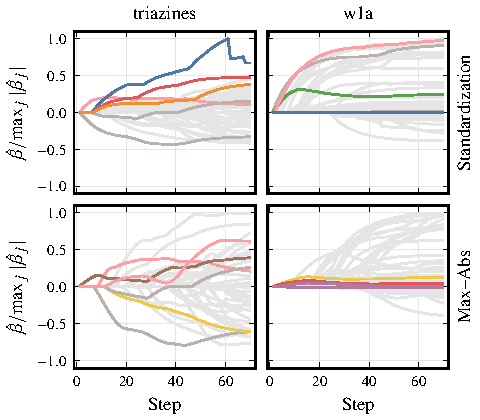
\includegraphics[]{plots/realdata_paths_small.pdf}
  \caption{%
    Lasso paths for real datasets using two types of normalization:
    standardization and maximum absolute value normalization (max--abs). We have fit
    the lasso path to two different datasets:
    \data{triazines}~\citep{king} and \data{w1a}~\citep{platt1998}. (See \Cref{sec:data-summary}
    for more information about these data sets.) For each
    dataset, we have colored the coefficients if they were among the first five
    to become non-zero under either of the two normalization schemes.
  }
  \label{fig:realdata-paths}
\end{figure}

In spite of this relationship between normalization and regularization, there has so far
been no research on the topic. Instead, the choice of normalization is often motivated by
being standard. And sometimes the choice is based on computational aspects such as
optimization performance and data storage. At the time of writing, for instance, the
popular machine learning library \texttt{scikit-learn}~\citep{scikit-learndevelopers2024}
recommends maximum absolute value normalization in the particular case of sparse data. Yet,
as we have already seen (\Cref{fig:realdata-paths}), this may have dramatic effects for the
results.

Standardization is a natural choice when the features are normally distributed. But for
other types of data the choice is not as straightforward. There is for instance no clear
approach to normalizing binary features (where the each observations takes either of only
two values). Anecdotal suggestions include not normalizing at all or to normalize as you
would if it were continuous data---the implications of either of these suggestions (or in
deed any other), however, have yet to be investigated.

In this paper we will begin to bridge this knowledge gap by studying normalization in the
context of binary data. We will focus on three models that each correspond to a particular
case of \Cref{eq:general-objective}: the lasso, ridge, and elastic net~\citep{zou2005}. The
latter of these, the elastic net, is a generalization of the previous two, and is
represented by the following optimization problem:
%
\begin{multline}
  \label{eq:elastic-net}
  \operatorname*{minimize}_{\beta_0 \in \mathbb{R},\vec{\beta} \in \mathbb{R}^p}\bigg( f(\beta_0, \vec{\beta};\vec{X},\vec{y},\lambda_1,\lambda_2)= \\
  \frac{1}{2} \lVert \vec y - \beta_0 - \tilde{\mat{X}}\vec{\beta} \rVert^2_2  + \lambda_1 \lVert \vec\beta \rVert_1 + \frac{\lambda_2}{2}\lVert \vec \beta \rVert_2^2\bigg).
\end{multline}
%
Setting \(\lambda_1 = 0\) results in the ridge regression objective, whereas \(\lambda_2 =
0\) gives us the lasso. These methods are staples in the field of statistics and machine
learning and are accompanied by a large body of theoretical work and applications for real
data.

We pay particular attention to the case when binary features are imbalanced, that is, have
relatively many ones or zeroes. In this scenario, we demonstrate that the choice of
normalization directly influences the estimated regression coefficients and that this
effect is different for the lasso and ridge regression. In the case of the lasso, we show
that this bias can be mitigated by scaling with variance but that this comes at the cost of
increased variance. For ridge regression we show that scaling by standard deviation
achieves the same effect. In the case of the elastic net, however, we show that there is no
simple normalization method that can mitigate this bias but that it is possible to
circumvent it by instead weighting the penalty terms in the elastic net.

We also study the case of mixed data and show that the choice of normalization has implicit
consequences for the relative weighting of binary and normal features, even in the case
when the binary features are balanced. If we believe, for instance, that a unit change in
the binary variable should equal a certain change in the normal variable (say, two standard
deviations), then scaling must be modified to take this into account.

% TODO: complete this paragraph
Finally, we look at a simple case of interactions between normal and binary features, and
demonstrate what?


\section{Preliminaries}

Throughout this paper, we assume that the data is generated from a linear model, \(y_i =
\beta_0^* + \vec x_i^\T \vec\beta^* + \varepsilon_i\) for \(i \in [n]\) where \([n] =
\{1,2,\dots,n\}\) and we use \(\beta_0^*\) and \(\vec\beta^*\) to denote the true intercept
and coefficients, respectively, and \(\varepsilon_i\) to denote measurement noise. \(\mat
X\) is the \(n \times p\) design matrix with features \(\vec x_j\) and \(\vec y\) the \(n
\times 1\) response vector. Furthermore, we use \(\hat\beta_0\) and \(\hat{\vec{\beta}}\)
to denote our estimates of the intercept and coefficients. We will also assume \(\mat{X}\),
\(\beta_0^*\), and \(\vec{\beta}^*\) to be fixed.

There is considerable ambiguity regarding key terms in the literature. Here, we define
\emph{normalization} as the process of centering and scaling the feature matrix, which we
now formalize.

\begin{definition}[Normalization]
  \label{def:normalization}
  Let \(\tilde{\mat X}\) be the normalized feature matrix with elements
  \(\tilde{x}_{ij} = (x_{ij} - c_{j})/s_j\), where \(x_{ij}\) is an element of
  \(\mat{X}\) and \(c_j\) and \(s_j\) are the \emph{centering} and
  \emph{scaling} factors respectively.
\end{definition}

% Some authors refer to the procedure in \Cref{def:normalization} as \emph{standardization},
% but here we define standardization only as the case when centering with the mean and
% scaling with the (uncorrected) standard deviation.

\subsection{Types of Normalization}

There are many different strategies for normalizing the design matrix. We list a few common
choices in \Cref{tab:normalization-types}. Standardization is perhaps the most popular type
of normalization, at least in the field of statistics. One of its benefits is that it
simplifies certain aspects of fitting the model, such as fitting the intercept. The
downside of standardization is that it involves centering by the mean, which destroys
sparsity. This is not a problem when \(\bm{X}\) is stored as a dense matrix; but when the
data is sparse, it may increase memory use and processing time.

% TODO: move to appendix?
\begin{table}[hbt]
  \centering
  \caption{
    Common ways to normalize a matrix of features using centering and scaling
    factors \(c_j\) and \(s_j\), respectively. Note that \(\bar{x}_j =
    n^{-1}\sum_{i=1}^n x_{ij}\).
  }
  \label{tab:normalization-types}
  \vskip 0.15in
  \small
  \begin{tabular}{lll}
    \toprule
    Normalization            & \(c_{j}\)          & \(s_j\)                                                   \\
    \midrule
    Standardization          & \(\bar{x}_j\)      & \(\sqrt{\frac{1}{n}\sum_{i=1}^n (x_{ij} - \bar{x}_j)^2}\) \\
    \addlinespace
    Max--Abs                 & 0                  & \(\max_i|x_{ij}|\)                                        \\
    \addlinespace
    Min--Max                 & \(\min_i(x_{ij})\) & \(\max_i(x_{ij}) - \min_i(x_{ij})\)                       \\
    \addlinespace
    \(\ell_1\)-Normalization & 0 or \(\bar{x}_j\) & \(\lVert \vec{x}_j\rVert_1\)                              \\
    \addlinespace
    Adaptive Lasso           & 0                  & \(\hat{\beta}_j^\text{OLS}\)                              \\
    \bottomrule
  \end{tabular}
\end{table}

When the data is sparse, a common alternative to standardization is to scale features by
their maximum absolute values (max--abs normalization). This method has no impact on binary
data\footnote{Except in the extreme case when all values are 0.} and therefore retains
sparsity. For other types of data, it scales the features to take values in the range
\([-1, 1]\). Since the scaling is determined by a single value for each feature, the method
is naturally sensitive to outliers. For many types of data, such as normally distributed
data, it is also often the case that the sample maximum depends on sample size, which often
makes use of the method problematic~(\Cref{thm:maxabs-gev}~(\Cref{sec:additional-theory})).

% TODO: should we study l1-normalization more?
Min-max normalization scales the data to lie in \([0, 1]\). As with the max--abs method,
min-max normalization retains sparsity and also shares its sensitivity to outliers and
sample size. Unlike max--abs scaling, however, min--max scaling is not sensitive to the
\emph{location} of the data, only its \emph{spread}. In \(\ell_1\)-normalization, each
feature is scaled with its sum of absolute value. The method is common in signal
processing. A special case of normalization is the adaptive lasso~\citep{zou2006}, which is
a two-step procedure. First we fit a model such as ordinary least-squares (OLS) or ridge
regression. Then we use the estimated coefficients to scale the features and refit.

\subsection{Lasso, Ridge, and Elastic Net Regression}%
\label{sec:elastic-net-solution}

If we include an intercept and assume that the features of the normalized design matrix are
orthogonal, that is, \(\tilde{\mat{X}}^\intercal \tilde{\mat{X}} =
\diag\left(\tilde{\vec{x}}_1^\T \tilde{\vec{x}}_1, \dots, \tilde{\vec{x}}_p^\intercal
\tilde{\vec{x}}_p\right) \), the solution to the coefficients in the elastic net problem is
given by
%
\begin{equation}
  \label{eq:orthogonal-solution-normalized}
  \hat{\beta}^{(n)}_j = \frac{\st_{\lambda_1}\left(\tilde{\vec{x}}_j^\T \vec{y}\right)}{\tilde{\vec{x}}_j^\T \tilde{\vec{x}}_j + \lambda_2},
  \qquad
  \hat{\beta}_0^{(n)} = \frac{\vec{y}^\T \ones}{n},
\end{equation}
%
where \(\st_\lambda(z) = \sign(z) \max(|z| - \lambda, 0)\) is the soft-thresholding
operator. (See \Cref{sec:elastic-net-estimator} for a derivation of this.)

Normalization changes the optimization problem and its solution, the coefficients, which
will now be on the scale of the normalized features. But we are interested in
\(\hat{\vec{\beta}}\): the coefficients on the scale of the original problem. To obtain
these, we transform the coefficients from the normalized poblem, \(\hat\beta^{(n)}_j\),
back via \(\hat\beta_j = \hat\beta^{(n)}_j/s_j\) for \(j \in [p]\). There is a similar
transformation for the intercept but we omit here since we are not interested in it.

\section{Bias and Variance of the Elastic Net Estimator}\label{sec:theory}

% TODO: write a table of the bias and variance formulations for each type instead.

Now, assume that \(\mat{X}\) is fixed and that \(\vec{y} = \mat{X}\vec{\beta} +
\vec{\varepsilon}\), where \(\varepsilon_i\) is identically and independently distributed
noise with mean zero and finite variance \(\sigma_\varepsilon^2\). As in the previous
section, we assume that the feature vectors are orthogonal. We are interested in the
expected value of \Cref{eq:orthogonal-solution}, \(\E \hat{\beta}_j\). Let
\[
  {Z_j} = \tilde{\vec{x}}_j^\T \vec{y} = \tilde{\vec{x}}_j^\T(\mat{X}\vec{\beta}^* + \vec{\varepsilon}) = \tilde{\vec{x}}_j^\T (\vec{x}_j\beta_j^* + \boldsymbol{\varepsilon})
  \qquad
  \text{and}
  \qquad
  d_j = s_j(\tilde{\vec{x}}_j^\T \tilde{\vec{x}}_j + \lambda_2)
\]
so that \(\hat{\beta}_j = \st_{\lambda_1}({Z_j})/d_j\). Since \(d_j\) is fixed under our
assumptions, we will direct most of our focus towards \(S_{\lambda_1}({Z_j})\). First
observe that
\[
  \begin{aligned}
    \tilde{\vec{x}}_j^\T \tilde{\vec{x}}_j & = \frac{1}{s_j^2}(\vec{x}_j - c_j)^\T (\vec{x}_j - c_j) = \frac{\vec{x}_j^\T\vec{x}_j - nc_j^2}{s^2_j} = \frac{n \nu_j}{s_j^2}, \\
    \tilde{\vec{x}}_j^\T \vec{x}_j         & = \frac{1}{s_j}(\vec{x}_j^\T \vec{x}_j - \vec{x}_j^\T \ones c_j) = \frac{n \nu_j}{s_j},
  \end{aligned}
\]
where \(\nu_j\) is the uncorrected sample variance of \(\vec{x}_j\). This means that
\begin{equation}
  \label{eq:z-d}
  {Z_j} = \frac{\beta_j^* n \nu_j- \vec{x}_j^\T \vec{\varepsilon}}{s_j}
  \qquad\text{and}\qquad
  d_j = s_j\left(\frac{n \nu_j}{s_j^2} + \lambda_2\right).
\end{equation}
For the expected value and variance of \({Z_j}\) we then have
\begin{align*}
  \E {Z_j}   & = \mu_j = \E \left( \tilde{\vec{x}}_j^\T (\vec{x}_j\beta^*_j + \vec{\varepsilon}) \right)  = \tilde{\vec{x}}_j^\T\vec{x}_j \beta^*_j = \frac{\beta_j^* n \nu_j}{s_j},            \\
  \var {Z_j} & = \sigma_j^2 = \var\left(\tilde{\vec{x}}_j ^\T \vec{\varepsilon}\right) = \tilde{\vec{x}}_j^\T \tilde{\vec{x}}_j\sigma_\varepsilon^2 = \frac{n\nu_j\sigma_\varepsilon^2}{s_j^2}.
\end{align*}

The expected value of the soft-thresholding estimator is
\begin{multline*}
  \E \st_\lambda({Z_j}) = \int_{-\infty}^\infty \st_\lambda(z) f_{Z_j}(z) \du z
  = \int_{-\infty}^\infty \ind{|z| > \lambda} (z -\sign(z)\lambda) f_{Z_j}(z) \du z
  \\= \int_{-\infty}^{-\lambda}(z + \lambda)f_{Z_j}(z) \du z + \int_{\lambda}^\infty (z - \lambda)f_{Z_j}(z) \du z.
\end{multline*}
And then the bias of \(\hat\beta_j\) with respect to the true coefficient \(\beta_j^*\) is
\begin{equation*}
  \E \hat\beta_j - \beta_j^* = \frac{1}{d_j}\E \st_\lambda({Z_j}) - \beta^*_j.
\end{equation*}

Finally, we note that the variance of the soft-thresholding estimator is
\begin{equation}
  \label{eq:st-variance}
  \var {S_\lambda({Z_j})} = \int_{-\infty}^{-\lambda}(z + \lambda)^2f_{Z_j}(z) \du z + \int_{\lambda}^\infty (z - \lambda)^2 f_{Z_j}(z) \du z - \left(\E \st_\lambda({Z_j})\right)^2
\end{equation}
and that the variance of the elastic net estimator is therefore
\begin{equation*}
  \var \hat\beta_j = \frac{1}{d_j^2} \var \st_\lambda({Z_j}).
\end{equation*}

\subsection{Normally Distributed Noise}

Next, we add the additional assumption that \(\vec{\varepsilon}\) is normally distributed.
Then
\[
  {Z_j} \sim \normal\left(\mu_j = \tilde{\vec{x}}_j^\T\vec{x}_j \beta_j, \sigma_j^2 = \tilde{\vec{x}}_j^\T\tilde{\vec{x}}_j \sigma_\varepsilon^2 \right).
\]
Let \(\theta_j = -\mu_j -\lambda_1 \) and \(\gamma_j = \mu_j - \lambda_1\). Then the
expected value of soft-thresholding of \({Z_j}\) is
\begin{align}
  \E \st_{\lambda_1}({Z_j}) & = \int_{-\infty}^\frac{\theta_j}{\sigma_j} (\sigma_j u - \theta_j) \pdf(u) \du u + \int_{-\frac{\gamma_j}{\sigma_j}}^\infty (\sigma_j u + \gamma_j) \pdf(u) \du u                                               \nonumber                              \\
                            & = -\theta_j \cdf\left(\frac{\theta_j}{\sigma_j}\right) - \sigma_j \pdf\left(\frac{\theta_j}{\sigma_j}\right) + \gamma_j \cdf\left(\frac{\gamma_j}{\sigma_j}\right) + \sigma_j \pdf\left(\frac{\gamma_j}{\sigma_j}\right) \label{eq:mean-centered-eval}
\end{align}
where \(\pdf(u)\) and \(\cdf(u)\) are the probability density and cumulative distribution
functions of the standard normal distribution, respectively.

Next, computing \Cref{eq:st-variance} gives
\begin{align}
  \label{eq:mean-centered-variance}
  % \int_{-\infty}^{-\lambda_1}(z+ \lambda_1)^2 f_{Z_j}(z) \du z
  % & = \sigma_j^2 \int_{-\infty}^{\frac{\theta_j}{\sigma_j}} y^2 \pdf(y) \du y + 2 \theta_j \sigma_j \int_{-\infty}^{\frac{\theta_j}{\sigma_j}} y \pdf(y) \du y + \theta_j^2 \int_{-\infty}^{\frac{\theta_j}{\sigma_j}} \pdf(y) \du y                                                                               \nonumber \\
  \var{S_\lambda(Z_j)} & = \frac{\sigma_j^2}{2} \left( \erf\left(\frac{\theta_j}{\sigma_j\sqrt{2}}\right) - \frac{\theta_j}{\sigma_j}\sqrt{\frac{2}{\pi}} \exp\left(-\frac{\theta_j^2}{2\sigma_j^2}\right) + 1 \right) + 2 \theta_j \sigma_j \pdf \left(\frac{\theta_j}{\sigma_j}\right) + \theta_j^2 \cdf\left(\frac{\theta_j}{\sigma_j}\right) \nonumber               \\
                       & \phantom{={}} + \frac{\sigma_j^2}{2} \left( \erf\left(\frac{\gamma_j}{\sigma_j\sqrt{2}}\right) - \frac{\gamma_j}{\sigma_j}\sqrt{\frac{2}{\pi}} \exp\left(-\frac{\gamma_j^2}{2\sigma_j^2}\right) + 1 \right) + 2 \gamma_j \sigma_j \pdf \left(\frac{\gamma_j}{\sigma_j}\right) + \gamma_j^2 \cdf\left(\frac{\gamma_j}{\sigma_j}\right) \nonumber \\
                       & \phantom{={}} - \big(\E \st_{\lambda_1}({Z_j})\big)^2.
\end{align}
Consequently, we can also
compute the mean-squared error via the bias-variance decomposition
\begin{equation*}
  \mse (\hat\beta_j, \beta^*_j) = \var\hat\beta_j + \left(\E \hat\beta_j - \beta^*_j\right)^2.
\end{equation*}

\subsection{Binary Features}\label{sec:theory-binary-features}

The main focus in this paper is the case when \(\vec{x_j}\) is a binary feature with class
balance \(q_j = \bar{\vec{x}}_j\), that is, \(x_{ij} \in \{0, 1\}\) for all \(i\) and
\(\sum_{i=1}^n x_{ij} = nq\). In this case, inserting \(\nu_j = (q_j - q_j^2)\) (the
uncorrected sample variance for a binary feature) into \Cref{eq:z-d}, we have
\[
  {Z_j} = \frac{\beta_j^* n(q_j - q_j^2) - \vec{x}_j^\T \vec{\varepsilon}}{s_j}
  ,\qquad
  d_j = s_j\left(\frac{n(q_j - q_j^2)}{s_j^2} + \lambda_2\right),
\]
% \[
%   \begin{aligned}
%     \tilde{\vec{x}}_j^\T \tilde{\vec{x}}_j & = \frac{1}{s_j^2}(\vec{x}_j - \ones c_j)^\T (\vec{x}_j - \ones c_j) = \frac{1}{s^2_j}(nq - 2nq_j^2 + nq_j^2) = \frac{nq_j(1-q_j)}{s^2_j}, \\
%     \tilde{\vec{x}}_j^\T \vec{x}_j         & = \frac{1}{s_j}(\vec{x}_j^\T \vec{x}_j - \vec{x}_j^\T \ones c_j) = \frac{nq_j(1 - q_j)}{s_j}.
%   \end{aligned}
% \]
and consequently
\[
  \mu_j = \frac{\beta^*_j n(q_j - q_j^2)}{s_j}\qquad \text{and} \qquad \sigma_j^2 = \frac{\sigma_\varepsilon^2n(q_j- q_j^2)}{s^2_j}.
\]
%
We obtain the expected value of the elastic net estimate with respect to \(q_j\) by
inserting \(\mu_j\) and \(\sigma_j\) into \Cref{eq:mean-centered-eval}.

The presence of the factor \(q_j - q_j^2\) in \(\mu_j\), \(\sigma_j^2\), and \(d_j\) means
that there is a link between class balance and the elastic net estimator and that this
relationship is mediated by the scaling factor \(s_j\). To achieve some initial intuition
for this relationship, we consider the noiseless case (\(\sigma_\varepsilon = 0\)) in
which, inserting \(\mu_j\) and \(d_j\) into \Cref{eq:orthogonal-solution} yields
\begin{equation}
  \label{eq:noiseless-estimator}
  \hat{\beta}_j = \frac{\st_{\lambda_1}(\tilde{\vec{x}}_j^\intercal \vec{y})}{s_j\left(\tilde{\vec{x}}_j^\intercal \tilde{\vec{x}}_j + \lambda_2\right)}
  =
  \frac{\st_{\lambda_1}\left(\frac{\beta_j^* n (q_j - q_j^2)}{s_j}\right)}{s_j\left(\frac{n(q_j - q_j^2)}{s_j^2} + \lambda_2\right)}.
\end{equation}
%
This expression shows that the class balance in fact affects the estimator directly. For
values of \(q_j\) close to \(0\) or \(1\), the input into the soft-thresholding part of the
estimator will diminish and consequently force the estimate to zero, that is, unless we use
the scaling factor \(s_j = q_j - q_j^2\), in which case the soft-thresholding part will be
unaffected by class imbalance. This choice will not, however, mitigate the impact of class
imbalance on the ridge part of the estimator, for which we would instead need \(s_j = (q_j
- q_j^2)^{1/2}\). For any other choices, \(q_j\) will affect the estimator through both the
ridge and lasso parts, which means that there exists no scaling \(s_j\) that will mitigate
the bias in this case. Later on in \Cref{sec:binary-weighting} we will show how to mitigate
this issue for the elastic net by scaling the coefficients in the penalty term. But for
now, we will continue to focus on case of normalization.

Based on these facts, we will consider the scaling parameterization \(s_j =
(q_j-q_j^2)^\delta\), \(\delta \geq 0\). This includes the cases that we are primarily
interested in, that is, \(\delta = 0\) (no scaling), \(\delta = 1/2\) (standard-deviation
scaling), and \(\delta = 1\) (variance scaling). Note that the last of these types,
variance scaling, is not a standard type of normalization; yet, as we have already seen, it
has some interesting properties in the context of binary features.

Another interesting fact about \Cref{eq:noiseless-estimator}, which holds also in the noisy
situation, is that even when the binary feature is balanced (\(q_j = 1/2\)), normalization
will still have an effect on the estimator. Using \(\delta = 0\), for instance, leads the
true coefficient \(\beta_j^*\) in the input to \(\st_\lambda\) to be scaled by \(n (q_j -
q_j^2) = n/4\). For \(\delta = 1\) there would in contrast be no scaling in the
class-balanced case. And for \(\delta = 1/2\), the scaling factor is \(n/2\). Generalizing
this we see that to achieve equivalent scaling in the class-balanced case for all types of
normalization, under our parameterization, we would need to use \(s_j = 4^{\delta - 1} (q_j
- q_j^2)^\delta\). But this only resolves the issue for the lasso. To achieve a similar
effect for ridge regression, we would need another (but similar) modification. Since all
features are binary under our current assumptions, however, we will for now just assume
that we scale \(\lambda_1\) and \(\lambda_2\) to account for this effect,\footnote{We do
  this in all of the following examples.} which is equivalent to modifying \(s_j\). We will
return to this issue later in \Cref{sec:mixed-data} where we consider mixes of binary and
normally distributed features, in which case this has significant implications.

% TODO: This makes it seem like it would make more sense to adjust λ instead of the scaling parameter to compensate for class balance.

We now leave the noise-less scenario and proceed to consider how class balance affects the
probability of selection, bias, and variance of the elastic net estimator, starting with
the first of these. A consequence of the normal error distribution and consequent normal
distribution of \({Z_j}\) is that the probability of selection in the elastic net problem
is given analytically by
\begin{align}
  \label{eq:selection-probability}
  \Pr\left(\hat{\beta}_j \neq 0\right) & = \Pr\left(\st_{\lambda_1}({Z_j}) \neq 0\right)                                                                                                                                                                                                                           \nonumber \\
                                       & = \Pr\left({Z_j} > \lambda_1\right) + \Pr\left({Z_j} < -\lambda_1\right)                                                                                                                                                                                                  \nonumber \\
                                       & = \cdf\left(\frac{\mu_j - \lambda_1}{\sigma_j}\right) + \cdf\left(\frac{- \mu_j -\lambda_1}{\sigma_j}\right)                                                                                                                                                              \nonumber \\
                                       & = \cdf \left( \frac{\beta_j^*n (q_j-q_j^2)^{1/2} - \lambda_1(q_j-q_j^2)^{\delta - 1/2}}{\sigma_\varepsilon \sqrt{n}}\right)                 + \cdf \left( \frac{-\beta_j^*n (q_j-q_j^2)^{1/2} - \lambda_1(q_j-q_j^2)^{\delta - 1/2}}{\sigma_\varepsilon \sqrt{n}}\right).
\end{align}

Letting \(\theta_j = -\mu_j - \lambda_1 \) and \(\gamma_j = \mu_j - \lambda_1\), we can
express the probability of selection in the limit as \(q_j \rightarrow 1^+\) as
\begin{equation}
  \label{eq:selection-probability-limit}
  \lim_{q_j \rightarrow 1^+} \Pr(\hat{\beta}_j \neq 0) =
  \begin{cases}
    0                                                                & \text{if } 0 \leq \delta < \frac{1}{2}, \\
    2\cdf\left(-\frac{\lambda_1}{\sigma_\varepsilon \sqrt{n}}\right) & \text{if } \delta = \frac{1}{2},        \\
    1                                                                & \text{if } \delta > \frac{1}{2}.
  \end{cases}
\end{equation}

In \Cref{fig:selection-probability}, we plot this probability for various settings of
\(\delta\) for a single feature. Our intuition from the noise-less case holds: \(\delta\)
mitigates the influence of class imbalance on selection probability. The lower the value of
\(\delta\), the larger the effect of class imbalance becomes. Note that the probability of
selection initially decreases also in the case when \(\delta \geq 1\). This is a
consequence of increased variance of \({Z_j}\) due to the scaling factor that scales the
measurement noise \(\sigma_\varepsilon^2\) upwards. Then, as \(q_j\) approaches 1, the
probability picks up again and eventually approaches 1 for \(\delta \in \{1, 1.5\}\). The
reason for this is that the variance of \({Z_j}\) eventually explodes (again due to the
scaling), which ultimately removes the soft-thresholding effect altogether. Note that the
selection probability is unaffected by \(\lambda_2\).

\begin{figure}[htpb]
  \centering
  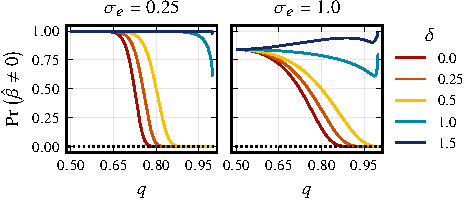
\includegraphics[]{plots/selection_probability.pdf}
  \caption{%
    Probability of selection in the lasso given a measurement noise level
    \(\sigma_\varepsilon\), a regularization parameter \(\lambda_1\), and a class balance
    \(q_j\). The scaling factor is set to \(s_j = (q_j - q_j^2)^\delta\), \(\delta
    \geq 0\). The dotted line represents the asymptotic limit for \(\delta = 1/2\) (the standardization case). \label{fig:selection-probability}}
\end{figure}

Now we turn to the impact of class imbalance on bias and variance of the elastic net
estimator. We begin, in \Cref{thm:classbalance-bias}, by considering the expected value of
the elastic net estimator in the limit as \(q_j \rightarrow 1^+\).

\begin{theorem}
  \label{thm:classbalance-bias}
  If \(\vec{x}_j\) is a binary feature with class balance \(q_j \in (0, 1)\), \(\lambda_1 \in [0,\infty)\), \(\lambda_2 \in [0,\infty)\), \(\sigma_\varepsilon > 0\), and \(s_j = (q_j - q_j^2)^{\delta}\), \(\delta \geq 0\)  then
  \[
    \lim_{q_j \rightarrow 1^+} \E \hat{\beta}_j =
    \begin{cases}
      0                                                                                                  & \text{if } 0 \leq \delta < \frac{1}{2}, \\
      \frac{2n \beta_j^*}{n + \lambda_2} \cdf\left(-\frac{\lambda_1}{\sigma_\varepsilon \sqrt{n}}\right) & \text{if } \delta = \frac{1}{2},        \\
      \beta^*_j                                                                                          & \text{if } \delta > \frac{1}{2}.
    \end{cases}
  \]
\end{theorem}

\Cref{thm:classbalance-bias} shows that the bias of the elastic net estimator when \(0 \leq
\delta < 1/2\) approaches \(-\beta_j^*\) as \(q_j \rightarrow 1^+\). Interestingly, when
\(\delta = 1/2\) (standardization), the estimate does not in fact tend to zero. Instead, it
approaches the true coefficient scaled by the probability that a standard normal variable
is smaller than \(\beta_j^*\sqrt{n}\sigma_\varepsilon^{-1}\). For \(\delta > 1/2\), the
estimate is unbiased asymptotically, which is related to the scaled variance of the error
term. Note that this unbiasedness is accompanied by exponentially increasing variance and
therefore also a rise in mean-squared error, and only serves to demonstrate that the cost
of the decoupling of \(q_j\) is unbearable in the large noise--large imbalance scenario. In
\Cref{thm:classbalance-variance}, we continue by studying the variance in the limit as
\(q_j \rightarrow 1^+\).

\begin{theorem}
  \label{thm:classbalance-variance}
  If \(\vec{x}_j\) is a binary feature with class balance \(q_j \in (0, 1)\) and \(\lambda_1,\lambda_2 \in (0,\infty)\), \(\sigma_\varepsilon > 0\), and \(s_j = (q_j - q_j^2)^{\delta}\), \(\delta \geq 0\), then
  \[
    \lim_{q_j \rightarrow 1^+} \var \hat{\beta}_j =
    \begin{cases}
      0      & \text{if } 0 \leq \delta < \frac{1}{2}, \\
      \infty & \text{if } \delta \geq \frac{1}{2}.
    \end{cases}
  \]
\end{theorem}

\begin{corollary}[Variance in Ridge Regression]
  \label{cor:ridge-variance}
  Assume the conditions of \Cref{thm:classbalance-variance} hold, except that \(\lambda_1 = 0\). Then
  \[
    \lim_{q_j \rightarrow 1^+} \var \hat{\beta}_j =
    \begin{cases}
      0                                          & \text{if } 0 \leq \delta < 1/4, \\
      \frac{\sigma_\varepsilon^2 n}{\lambda_2^2} & \text{if } \delta = 1/4,        \\
      \infty                                     & \text{if } \delta > 1/4.
    \end{cases}
  \]
\end{corollary}

\Cref{thm:classbalance-variance} formally proves the asymptotic variance effects of our
scaling parameter \(s_j\) which we have already discussed in the context of selection
probability and bias. Taken together with the results from \Cref{thm:classbalance-bias},
this suggests that the choice of scaling parameter, at least in the case of our specific
parameterization, introduces a bias--variance tradeoff with respect to \(\delta\): to
reduce bias (with respect to \(q_j\)), we need to pay the cost of increased variance.

In \Cref{fig:bias-var-onedim-lasso}, we now visualize bias, variance, and mean-squared
error for ranges of class balance and various noise-level settings for a lasso problem. The
figure demonstrates the bias--variance tradeoff that our asymptotic results suggested and
indicates that the optimal choice of \(\delta\) is related to the noise level in the data.
Since this level is unknown for most data sets, it suggests there might be value in
selecting \(\delta\) through hyper-optimization as is typically done for the other
hyper-parameters in the elastic net \((\lambda_1, \lambda_2)\)

\begin{figure}[htpb]
  \centering
  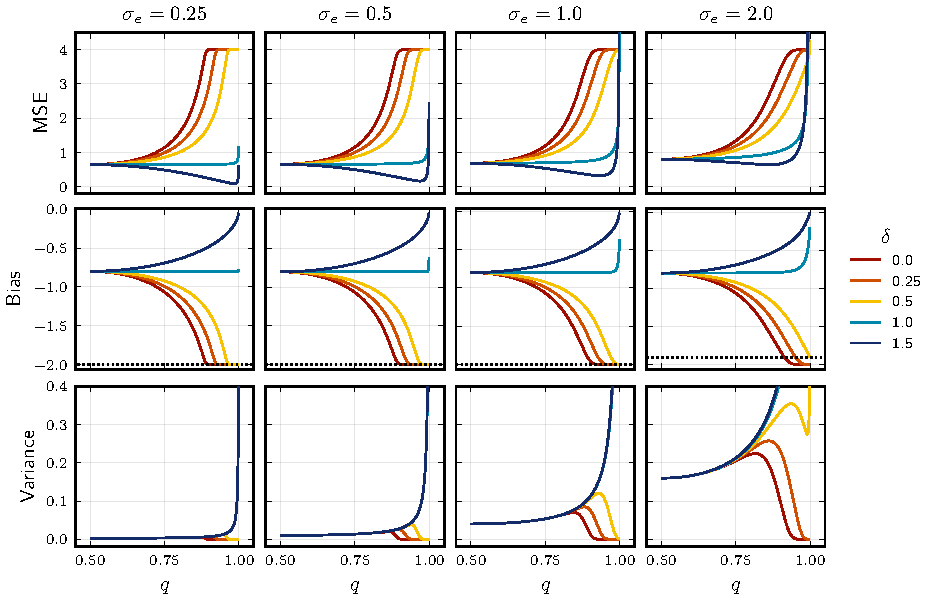
\includegraphics[]{plots/binary_onedim_bias_var_lasso.pdf}
  \caption{%
    Bias, variance, and mean-squared error for a one-dimensional lasso problem. We show these
    measures for various noise levels (\(\sigma_\varepsilon\)), class balances (\(q_j\)), and
    scaling factors (\(\delta\)). The dotted lines represent the asymptotic bias of the lasso
    estimator in the case of \(\delta = 1/2\). } \label{fig:bias-var-onedim-lasso}
\end{figure}

\begin{figure}[htpb]
  \centering
  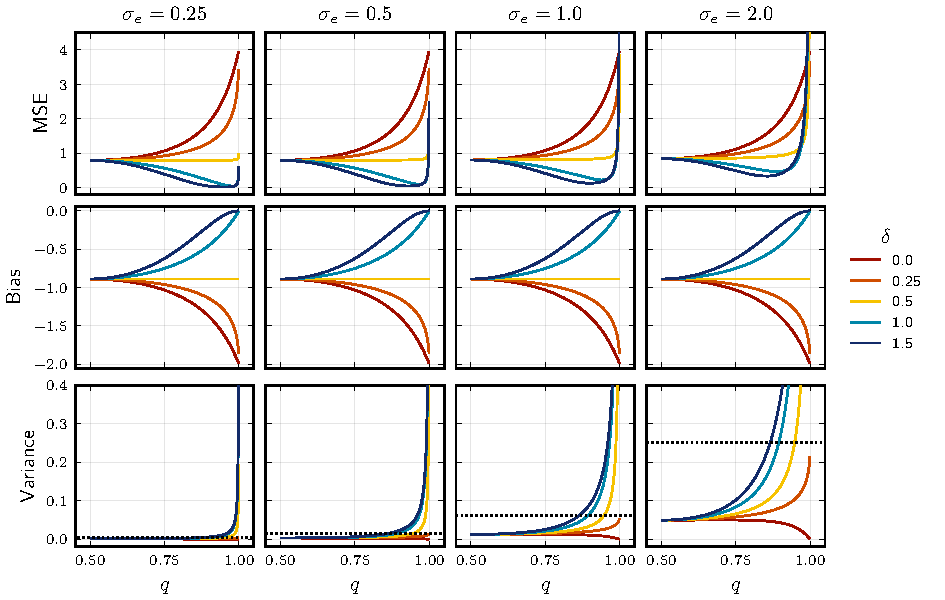
\includegraphics[]{plots/binary_onedim_bias_var_ridge.pdf}
  \caption{%
    Bias, variance, and mean-squared error for one-dimensional ridge regression. We show these
    measures for various noise levels (\(\sigma_\varepsilon\)), class balances (\(q_j\)), and
    scaling factors (\(\delta\)). The dotted lines represent the asymptotic bias of the lasso
    estimator in the case of \(\delta = 1/2\). } \label{fig:bias-var-onedim-ridge}
\end{figure}

So far, we have only considered a single binary feature. But under the assumption of
orthogonal features, it is straightforward to introduce multiple binary features. In a
first example, we study how the power of correctly detecting \(k=10\) signals under \(q_j\)
linearly spaced in \([0.5, 0.99]\)~(\Cref{fig:binary-power}). We set \(\beta^*_j = 2\) for
each of the signals, use \(n = 100\,000\), and let \(\sigma_\varepsilon = 1\). The level of
regularization is set to \(\lambda_1 = n 4^\delta/10\). As we can see, the power is
directly related to \(q_j\) and for unbalanced features stronger the higher the choice of
\(\delta\) is.

We also consider a version of the same setup, but with \(p\) linearly spaced in \([20,
    100]\) to compute the normalized mean-squared error (NMSE) and false discovery rate
(FDR)~(\Cref{fig:binary-fdr-mse}). As before, we let \(k = 10\) and consider three
different levels of class imbalance. The remaining \(p-k\) features have class balances
spaced evenly on a logarithmic scale from 0.5 to 0.99. Unsurprisingly, the increase in
power gained from selecting \(\delta = 1\) imposes increased false discovery rates. The
mean-squared error depends on the class balance. For class-balanced signals, \(\delta \in
\{0, 1/2\}\) proves to b the best choice, while for unbalanced signals, \(\delta = 1\) is
the best choice. In the case when \(q_j = 0.99\), the model under scaling with \(\delta =
0\) is altogether unable to detect any of the true signals, instead picking up on the
noisy, but better-balanced, features.

\begin{figure}[htpb]
  \centering
  \subcaptionbox{%
    The power (probability of detecting all true signals) of the lasso. In our orthogonal
    setting, power is constant over \(p\), which is why we have omitted the parameter in the
    plot. \label{fig:binary-power}
  }{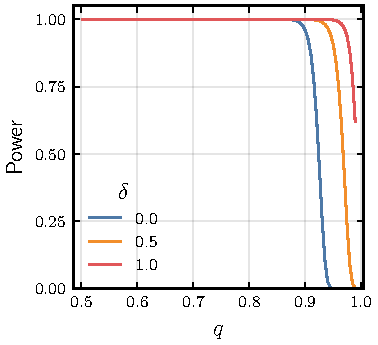
\includegraphics[]{plots/power.pdf}}\hfill%
  \subcaptionbox{%
    NMSE and FDR: the rate of coefficients incorrectly set to non-zero (false discoveries) to
    the total number of estimated coefficients that are nonzero (discoveries).
    \label{fig:binary-fdr-mse} }{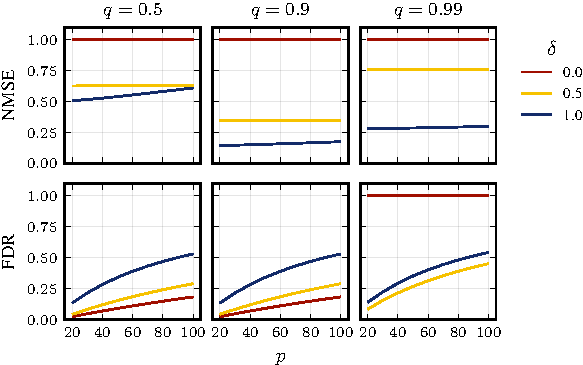
\includegraphics[]{plots/fdr_mse.pdf}}%%
  % 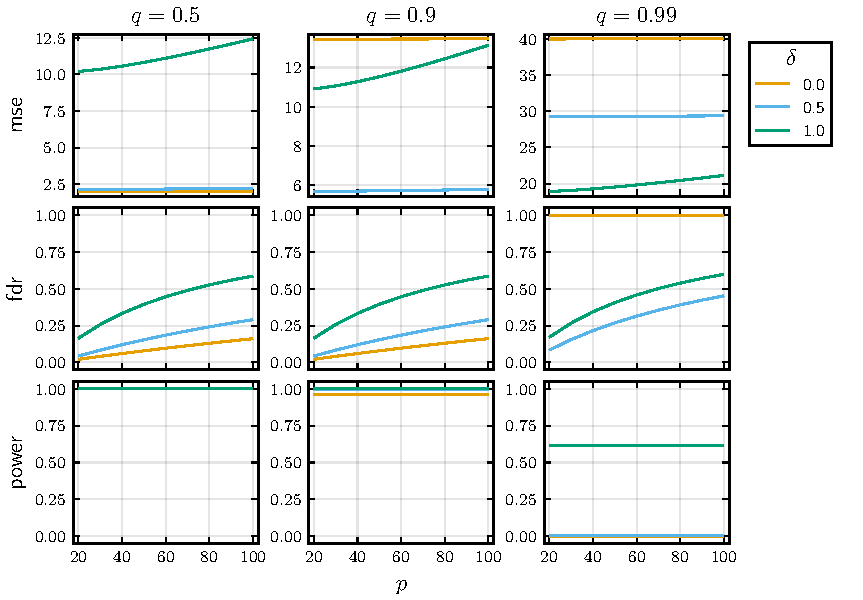
\includegraphics[]{plots/beta-bias-multidim.pdf}
  \caption{%
    Normalized mean-squared error (NMSE), false discovery rate (FDR), and power for a lasso problem with
    \(k = 10\) true signals (nonzero \(\beta_j^*\)), varying \(p\), and \(q_j \in [0.5, 0.99]\). The noise level is set at \(\sigma_\varepsilon = 1\) and \(\lambda_1 = 0.02\).
  }
\end{figure}

In \Cref{sec:experiments}, we will continue to study binary features in simulated
experiments. For now, however, we will turn to the case of mixed data.

\subsection{Mixed Data}\label{sec:mixed-data}

In this section, we consider the case where the features are made up of a mix of continuous
and and binary features. Throughout the section, we will continue to assume that
\(\mat{X}\) is fixed and that the features are orthogonal to one another. As in our
theoretical results, we will also restrict our focus to the case where the continuous
features are normally distributed.

A fundamental problem in the context of mixed data is how to put the binary and normal
features on the same scale, which we need to do in order for regularization to be, roughly
speaking, ``fair'', given that the solution is sensitive to the scale of the features. In
essence, we need to say something about how an effect associated with a one-unit change in
the binary feature (a flip) relates to a one-unit change in the continuous feature. Since
we assume our continuous feature to be normal, however, we will instead reason about change
in terms of standard deviations of the normal feature.

To setup this situation more formally, we will say that the effect of a binary feature
\(\vec{x}_1\) and a normal feature \(\vec{x}_2\) are \emph{comparable} if
\[
  \beta^*_1 = \kappa \sigma_{2}\beta^*_2,
\]
where \(\sigma_2\) is the standard deviation of \(\vec{x}_2\) and \(\kappa > 0\) is a
scaling factor that represents the number of standard deviations (of the continuous
feature) we consider achieves comparability between the features' effects. (Note that
\(\sigma_2 \beta_2^*\) is just the standardized coefficient for the normal feature.) We
illustrate this notion of comparability by the following examples.

\begin{example}
  Assume \(\kappa = 2\). If \(\vec{x}_2\) is sampled from \(\normal(\mu_j, 1/2^2)\), then the effects of \(\vec{x}_1\) and \(\vec{x}_2\) are comparable if \(\beta_1^* = \beta_2^*\).
\end{example}
\begin{example}
  Assume \(\kappa = 1\). If \(\vec{x}_2\) is sampled from \(\normal(\mu_j, 2^2)\), then the effects of \(\vec{x}_1\) and \(\vec{x}_2\) are comparable if \(\beta_1^* = 2\beta_2^*\).
\end{example}

Note that this definition refers to the data-generating mechanism, and not the regularized
estimates. What we ultimately want for comparability, however, is for the following
relationship to hold:
\[
  \hat{\beta}_1 = \kappa \sigma_{2}\hat{\beta}_2.
\]
Put plainly, we want the effects of regularization to be distributed evenly across the
estimates. The crux of the problem is how to choose the scaling factor \(s_j\) for the
binary features in order to achieve this effect for a given \(\kappa\). Let us assume that
we have two features, \(\vec{x}_1\) and \(\vec{x}_2\), where \(\vec{x}_1\) is binary and
\(\vec{x}_2\) is normally distributed and that their effects are comparable in the sense
given above. Then it should hold that
%
\begin{alignat}{3}
  \label{eq:comparable-effects}
  \hat{\beta}_1                                                                                                                          & = \kappa \sigma_2\hat{\beta}_2                                                                                                                           & \implies \nonumber \\
  \frac{\st_{\lambda_1}(\tilde{\vec{x}}_1^\intercal \vec{y})}{s_1\left(\tilde{\vec{x}}_1^\intercal \tilde{\vec{x}}_1 + \lambda_2\right)} & = \frac{\kappa \sigma_2 \st_{\lambda_1}(\tilde{\vec{x}}_2^\intercal \vec{y})}{s_2\left(\tilde{\vec{x}}_2^\intercal \tilde{\vec{x}}_2 + \lambda_2\right)} & \implies \nonumber \\
  \frac{\st_{\lambda_1}\left(\frac{n\beta_1^* (q - q^2)}{s_1}\right)}{s_1\left(\frac{n(q - q^2)}{s_1^2} + \lambda_2\right)}              & = \frac{\kappa \st_{\lambda_1}\left(\frac{n\beta_1^*}{\kappa} \right)}{n + \lambda_2}
\end{alignat}
%
since we standardize he normal feature and therefore \(s_2 = \sigma_2\).
% First observe that there is no simple function \(s_j\) for which \Cref{eq:comparable-effects} holds in general (\(q \in [0, 1]\), \(\lambda_1,\lambda_2 \in \mathbb{R}^+\)). 
For the lasso (\(\lambda_2 = 0\)) and ridge regression (\(\lambda_1=0\)), we observe that
\(s_1 = \kappa (q - q^2)\) and \(s_1 = (q - q^2)^{1/2}\), respectively, are the values for
which \Cref{eq:comparable-effects} hold. In other words, we can achieve comparability in
the lasso by scaling each binary feature with its variance times \(\kappa\), the number of
standard deviations we consider achieves comparability between the features' effects. And
for ridge regression, we can achieve comparability by scaling with standard deviation,
irrespective of \(\kappa\).

% For other choices of \(\lambda_1\), \(\lambda_2\), and \(\delta\), we can only achieve comparability for a specific level of class balance, and never for \(\lambda_1 >0\), \(\lambda_2 >0\).
For any other choices of \(s_1\), equality can only hold for a specific level of class
balance. If we let this level be \(q_0\), then, to achieve equality for \(\lambda_2 = 0\),
we need \(s_1 =\kappa (q_0 - q_0^2)^{1 - \delta}(q - q^2)^\delta\). Similarly, for
\(\lambda_1 = 0\), we need \(s_1 = (q_0 - q_0^2)^{1 - 2\delta} (q - q^2)^\delta\). In the
sequel, we will assume that \(q_0 = 1/2\), to have effects be equivalent for the
class-balanced case.

Note that this also means that there is an implicit relationship between the strength of
penalization for binary and normal features, which depends on the level of class balance
and normalization type. This means, for instance, that even in the class-balanced case (\(q
= 1/2\)), we have to account for the type of normalization if we want binary and normal
features to be treated equally. For example, if we were to use \(\delta=0\) and fit the
lasso, then \Cref{eq:comparable-effects} for a binary feature with \(q=1/2\) becomes
\[
  \frac{4\st_{\lambda_1}\left(\frac{n\beta_1^*}{4}\right)}{n}               = \frac{\kappa \st_{\lambda_1}\left(\frac{n\beta_1^*}{\kappa} \right)}{n},
\]
which then implies \(\kappa = 4\), which may or may not agree with our assumptions about
comparability between these features' effects.

For the rest of this paper, we will use \(\kappa = 2\). That is, we will say that the
effects are comparable if the effect of a flip in the binary feature equals the effect of a
two-standard deviation change in the normal feature. We base this argument on the
discussion by \citet{gelman2008}, who argues that the classical approach of comparing
standardized coefficients\footnote{Coefficients multiplied by the standard deviation of the
  respective feature.} awards effects of continuous features undue strength for most real
data, since a change from, for instance, the lower to the upper 16\% of the distribution
will equal approximately twice the effect of a change in the binary feature. Using two
standard deviations as a comparability factor would, in contrast, equivocate this change
with the flip of the binary feature, which we believe is a better default. We want to
stress that the choice of \(\kappa\) should, if possible, in general be made on a
case-by-case (feature-by-feature) basis, using all available knowledge about the data at
hand. But, irrespective of this, we also want to emphasize that the choice should be made.
If you do not make it explicitly, then it will be implicitly dictated through the
combination of normalization and penalization types you use.

Finally, note that the reasoning of comparability above rests on the assumption of no
noise. And we are, in fact, in general instead more interested in the expected value of the
estimators, which depend on the noise level. In the case of large class-imbalances and
large noise, for instance, our previous results (see \Cref{fig:bias-var-onedim-lasso} for
instance), suggest that the estimators for normally distributed and binary features will
not be comparable in this case.

% TODO: Say something about over and undersampling.

\subsection{The Elastic Net, and Penalty Weighting}\label{sec:binary-weighting}

We have so far shown that certain choices of scaling can mitigate the class-balance bias
imposed by the lasso and ridge regression. But we have also demonstrated in
\Cref{sec:theory-binary-features} that there is no choice of scaling in the case of the
elastic net that can achieve the same effect. \Cref{eq:noiseless-estimator}, however,
suggests a natural alternative to normalization, which is to use the weighted elastic
net~(\Cref{sec:weighted-elasticnet}) and weight the coefficients in the penalty term. We
can then control class-balance bias by setting our weights according to \(u_j = v_j = (q_j
- q_j^2)^{\omega}\), and counteract it, at least in the noiseless case, with \(\omega =
1\). For the lasso and ridge regression, this is equivalent to using \(\delta = 1\) and
\(\delta = 1/2\) respectively.

Results analagous to those in \Cref{sec:theory-binary-features} can be attained with a few
small modification for the weighted elastic net case. Starting with selection probablity,
we can set \(s_j = 1\) and replace \(\lambda_1\) with \(\lambda_1 u_j =
\lambda_1(q_j-q_j^2)^\omega\) in \Cref{eq:selection-probability}, which shows that
\(\omega\) and \(\delta\) have interchangeable effects for selection probability. Naturally
this extends to the limit in \Cref{eq:selection-probability-limit} as well.

As far as expected value and variance of the weighted elastic net estimator is concerned,
the quantities in \Cref{eq:mean-centered-eval} and \Cref{eq:mean-centered-variance} apply
directly in the case of the weighted elastic net given \(s_j = 1\) for all \(j\) and
replacing \(\lambda_1\) as in the previous paragraph and \(\lambda_2\) with \(\lambda_2
(q_j - q_j^2)^\omega\). On the other hand, the asymptotic results differ slightly as we
will show next, starting with the expected value.

\begin{theorem}
  \label{thm:weighted-elasticnet-bias}
  Let \(\vec{x}_j\) be a binary feature with class balance \(q_j \in (0, 1)\) and take
  \(\lambda_1 > 0\), \(\lambda_2 > 0\), and \(\sigma_\varepsilon > 0\). For the
  weighted elastic net with weights \(u_j = v_j = (q_j-q_j^2)^\omega\) and \(\omega \geq 0\), it holds that
  \[
    \lim_{q_j \rightarrow 1^+} \E \hat{\beta}_j =
    \begin{cases}
      0                              & \text{if } 0 \leq \omega < 1, \\
      \frac{\beta^*n}{n + \lambda_2} & \text{if } \omega = 1,        \\
      \beta^*                        & \text{if } \omega > 1.
    \end{cases}
  \]
\end{theorem}

This result is similar to the one for the unweighted but normalized elastic net. The only
difference arises in the case when \(\omega = 1\), in which case the limit is unaffected by
\(\lambda_1\) in the case of the weighted elastic net.

\begin{theorem}
  \label{thm:weighted-elasticnet-variance}
  Let \(\vec{x}_j\) be a binary feature with class balance \(q_j \in (0, 1)\) and take
  \(\lambda_1 > 0\), \(\lambda_2 > 0\), and \(\sigma_\varepsilon > 0\). For the
  weighted elastic net with weights \(u_j = v_j = (q_j-q_j^2)^\omega\) and \(\omega \geq 0\), it holds that
  \[
    \lim_{q_j \rightarrow 1^+} \var \hat{\beta}_j =
    \begin{cases}
      0      & \text{if } 0 \leq \delta < \frac{1}{2}, \\
      \infty & \text{if } \delta \geq \frac{1}{2}.
    \end{cases}
  \]
\end{theorem}

This result mimics the result for asymptotic variance in the case of the unweighted elastic
net.

In \Cref{fig:binary-onedim-bias-var-elnet}, we plot bias, variance, and mean-squared error
for the weighted elastic net. Again, we see that the asymptotic behavior of bias as \(q_j
\rightarrow 1^+\) depends on the noise level and that there is a

\begin{figure}[htpb]
  \centering
  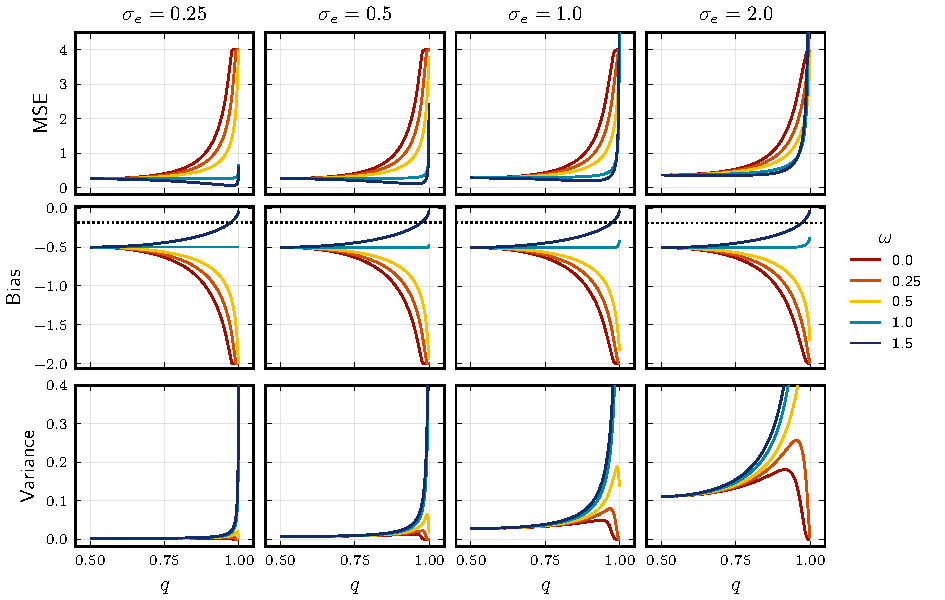
\includegraphics[]{plots/binary_onedim_bias_var_elnet.pdf}
  \caption{%
    Bias, variance, and mean-squared error in the case of the one-dimensional weighted elastic
    net. The measures are shown for different noise levels (\(\sigma_\varepsilon\)), class
    balances (\(q_j\)), and values of (\(\omega\)), which controls the weights that are set to
    \(u_j = v_j = 2\times 4^{\omega - 1}(q-q^2)^\omega\) in order for the results to be
    comparable across different values of \(\omega\). The dotted lines represent the asymptotic
    bias of the estimator in the case of \(\omega = 1\). In the case of \(\omega > 1\), the
    limit of the bias is zero. \label{fig:binary-onedim-bias-var-elnet}
  }
\end{figure}

As in the previous section \Cref{sec:mixed-data}, we modify the weighting factor to account
for the comparability relationship we want between binary and normal features.

\section{Experiments}

In the following sections we present the results of our experiments. For all simulated data
we generate our response vector according to \(\vec{y} = \mat{X}\vec{\beta}^* +
\vec{\varepsilon},\) with \(\vec{\varepsilon} \sim \normal(\vec{0}, \sigma_\varepsilon^2
\mat{I})\). We consider two types of features: binary (quasi-Bernoulli) and quasi-normal
features. To generate binary vectors, we sample \(\ceil{nq_j}\) indexes uniformly at random
without replacement from \([n]\) and set the corresponding elements to one and the
remaining ones to zero. To generate quasi-normal features, we generate a linear sequence
\(\vec{w}\) with \(n\) values from \(10^{-4}\) to \(1 - 10^{-4}\), set \(x_{ij} =
\cdf^{-1}(w_i)\), and then shuffle the elements of \(\vec{x}_j\) uniformly at random.

We use a coordinate descent solver to optimize our models, which we have based on the
algorithm outlined by \citet{friedman2010}. All experiments were coded using the Julia
programming language~\citep{bezanson2017} and the code is available at
\url{https://github.com/jolars/normreg}.
% in the supplementary material. 
All simulated experiments were run for at least 100 iterations and, unless stated
otherwise, are presented as means $\pm$ one standard deviation (using bars or ribbons).

\subsection{Normalization in the Lasso and Ridge Regression}%
\label{sec:experiments-lassoridge}

In this section we consider fitting the lasso and ridge regression to normalized data sets.
To normalize the data, we use standardize all quasi-normal features. For binary features,
we center by mean and scale by \(s_j \propto (q_j-q_j^2)^\delta\).
% where \(\delta = 0\)
% corresponds to no scaling, \(\delta = 1/2\) to standardization, and \(\delta = 1\) to
% variance scaling.

\subsubsection{Variability and Bias in Estimates}

In our first experiment, we consider fitting the lasso to a simulated data set with
\(n=500\) observations and \(p = \num{1000}\) features, out of which the first 20 features
correspond to signals, with \(\beta_j^*\) decreasing linearly from 1 to 0.1. We introduce
dependence between the features by copying the first \(\ceil{\rho n/2}\) values from the
first feature to each of the following features. In addition, we set the class balance of
the first 20 features so that it decreases linearly on a log-scale from 0.5 to 0.99. We
estimate the regression coefficients using the lasso, setting \(\lambda_1 = 2
\sigma_\varepsilon \sqrt{2 \log p }\).

The results~(\Cref{fig:binary-decreasing}, and \Cref{fig:binary-decreasing-full} in
\Cref{sec:additional-results-biasvar}) show that class balance has considerable effect,
particularly in the case of no scaling (\(\delta = 0\)), which corroborates our theory from
\Cref{sec:theory-binary-features}. At \(q_j=0.99\), for instance, the estimate
(\(\hat{\beta}_{20}\)) is consistently zero when \(\delta = 0\). For \(\delta=1\), we see
that class imbalance increases the variance of the estimates. What is also clear is that
the variance of the estimates increase with class imbalance and that this effect increases
together with \(\delta\).

\begin{figure}[htpb]
  \centering
  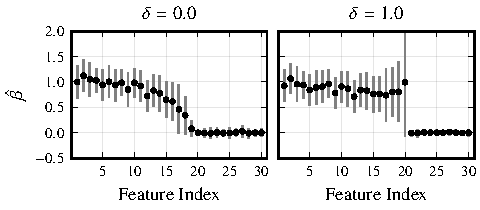
\includegraphics[]{binary_decreasing_small.pdf}
  \caption{%
    Regression coefficients for a lasso problem with binary data where \(n = 500\) and
    \(p = \num{1000}\) with 20 true signals. Here we show only the first 30
    coefficients. See \Cref{sec:experiments-lassoridge} for more information
    on the setup of this experiment.
  }
  \label{fig:binary-decreasing}
\end{figure}

\subsubsection{Predictive Performance}

In this section we examine the influence of normalization on predictive performance for
three different data sets: \data{a1a}~\citep{becker1996}, \data{rhee2006}~\citep{rhee2006},
and \data{w1a}~\citep{platt1998}.\footnote{See \Cref{sec:data-summary} for details about
  these data sets.} We evaluate performance in terms of normalized mean-squared error~(NMSE)
for lasso and ridge regression across a two-dimensional grid of \(\delta\) and \(\lambda\),
where for \(\delta\) we use a linear sequence from 0 to 1, and for \(\lambda\) a geometric
sequence from \(\lambda_\text{max}\) (the value of \(\lambda\) at which the first feature
enters the model) to \(10^{-2}\lambda_\text{max}\). We split the data into equal training
and validation set splits and for each combination of \(\lambda\) and \(\delta\) fit the
lasso or ridge to the training set.

We present the results for ridge regression in \Cref{fig:hyperopt-contours}, which shows
contour plots of the validation set error. We see that optimal setting of \(\delta\)
differs between the different data sets, suggesting that it is useful to choose \(\delta\)
by hyperparameter optimization. See
\Cref{fig:hyperopt-contours-full}~(\Cref{sec:predictive-performance-simulated}) for a plot
that includes the lasso as well.

% For
% \data{a1a}, the lasso is generally quite insensitive to the type of normalization, even if
% the optimal value is around 0.2. For ridge regression, lower values of \(\delta\) clearly
% work better. With the \data{w1a} data set, however, the relationship is flipped in the case
% of ridge regression and the optimal value is approximately 0.8. In the case of the lasso
% (for \(\data{w1a}\)), a value around 0.5 is optimal and low values (little scaling) yield
% worse prediction errors. Finally, for \data{rhee2006}, the lasso is again insensitive to
% normalization type. This is not the case for ridge, however, where a value around 0.2 is
% optimal and high values of \(\delta\) yield worse prediction errors.

\begin{figure}[htpb]
  \centering
  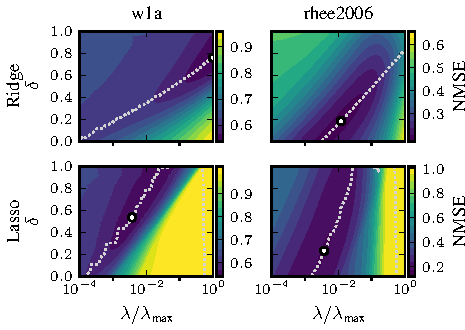
\includegraphics[]{hyperopt_surfaces_small.pdf}
  \caption{%
    Contour plots of normalized validation set mean-squared error (NMSE)
    for \(\delta\) and \(\lambda\) in ridge regression on
    three real data sets. The
    dotted path shows the smallest NMSE as a function of \(\lambda\) and the circles mark
    combinations with the lowest error.
  }
  \label{fig:hyperopt-contours}
\end{figure}

% We would like to point out that there is a dependency between \(\lambda\) and \(\delta\)
% that make it difficult to interpret the relationship between them and the error. This comes
% from the fact that scaling with a smaller value (as in \(\delta = 1\)) increases the sizes
% of the vectors, which means that the level of penalization is relaxed, relatively speaking.

In \Cref{sec:predictive-performance-simulated}, we extend these results with experiments on
simulated data under various class balances and signal-to-noise ratios, again showing that
normalization has an impact on predictive preformance.

\subsubsection{Mixed Data}\label{sec:experiments-mixed-data}

In \Cref{sec:mixed-data} we showed theoretically that care needs to be taken when
normalizing mixed data. Here we verify the theory through simulations. We construct a
quasi-normal feature with mean zero and standard deviation 1/2 and a binary feature with
varying class balance \(q_j\). We set the signal-to-noise ratio to 0.5 and use \(n =
\num{1000}\). These features are constructed so that their effects are comparable under the
notion of comparability that we introduced in \Cref{sec:mixed-data} using \(\kappa = 2\).
In order to preserve the comparability for the baseline case when we have perfect class
balance, we scale by \(s_j = 2 \times (1/4)^{1-\delta}(q_j-q_j^2)^\delta\). Finally, we set
\(\lambda\) to \(\lambda_\text{max}/2\) and \(2\lambda_\text{max}\) for lasso and ridge
regression respectively.

The results~(\Cref{fig:lasso-ridge-comparison}) reflect our theoretical results from
\Cref{sec:theory}. In the case of the lasso, we need \(\delta =1\) (variance scaling) to
avoid the effect of class imbalance, whereas for ridge we instead need \(\delta =1/2\)
(standardization). As our theory suggests, this extra scaling mitigates this class-balance
dependency at the cost of added variance.
% Note that we do not see the bias reduction that
% we observed in our theoretical results for high \(q_j\) values and \(\delta \geq 1/2\) in
% \Cref{fig:lasso-ridge-comparison}. This is related to the error term (signal-to-noise
% ratio) and level of \(q_j\). We would need stronger class imbalance and larger error for
% the effect to show up here.

\begin{figure}[htpb]
  \centering
  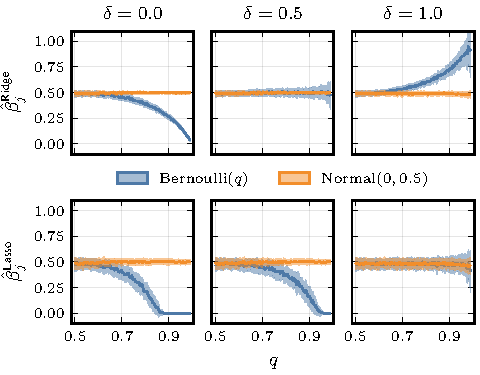
\includegraphics{mixed_data.pdf}
  \caption{%
    Lasso and ridge estimates for a two-dimensional problem where one feature is a binary
    feature with class balance \(q_j\) (\(\bernoulli(q_j)\)) and the other is quasi-normal
    with standard deviation 1/2, (\(\normal(0, 0.5)\)).
  }
  \label{fig:lasso-ridge-comparison}
\end{figure}

\subsubsection{Interactions}\label{sec:experiments-interactions}

Next, we study the effects of normalization and class balance on interactions in the lasso.
Our example consists of a two-feature problem with an added interaction term given by
\(x_{i3} = x_{i1}x_{i2}\). The first feature is binary with class balance \(q\) and the
second quasi-normal with standard deviation 0.5. We use \(n=1000\), \(\lambda_1 = n/4\),
and normalize the binary feature by mean-centering and scaling by \(\kappa (q - q^2)\),
using \(\kappa = 2\). We consider two different strategies for choosing \(s_3\): in the
first strategy, which we call \emph{Strategy 1}, we simply standardize the resulting
interaction feature.
% TODO: make a reference to where this is done
In the second strategy, \emph{Strategy 2} we center with mean and scale with \(s_1s_2\)
(the product of the scales of the binary and normal features).

The results for \(\bm{\beta}^* = \bm{1}\)~(\Cref{fig:interactions}) show that only strategy
2 estimates the effect of the interaction correctly. Strategy 1, meanwhile, only selects
the correct model if the class balance of the binary feature is close to 1/2 and in general
shrinks the coefficient too much. See
\Cref{fig:interactions-full}~(\Cref{sec:additional-experiments-interactions}) for results
on different choices of \(\bm{\beta}^*\).

\begin{figure}[htpb]
  \centering
  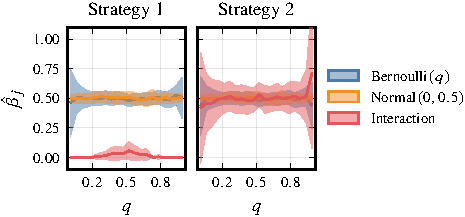
\includegraphics[]{interactions-classbalance-small.pdf}
  \caption{%
    Lasso estimates for a problem with a binary feature, a quasi-normal feature, and
    an interaction feature. We have set \(\bm{\beta}^* = \bm{1}\) and use two different normalization strategies where
    Strategy 1 represents standardization and Strategy 2 is mean-centering
    together with scaling by \(s_1 s_2\).
  }
  \label{fig:interactions}
\end{figure}

\subsection{The Weighted Elastic Net}

The weighted elastic net can be used as an alternative to normalization to correct for
class balance bias when \(\lambda_1 > 0\) and \(\lambda_2 >0\). To simplify the
presentation, we parameterize the elastic net as \(\lambda_1 = \alpha \lambda \) and
\(\lambda_2 = (1-\alpha) \lambda\), so that \(\alpha\) controls the balance between the
ridge and lasso. We conduct an experiment with the same setup as in
\Cref{sec:experiments-mixed-data}, but here we use the weighted elastic net instead with
\(\alpha = 0.5\) (See \Cref{sec:additional-experiments-weighted-elnet} for results using
other setting for \(\alpha\)). We use \(n=1000\) and vary \(\omega\), using the weights
\(u_j = v_j = (q_j - q_j^2)^{\omega}\) as we suggested in \Cref{sec:binary-weighting}. Our
results (\Cref{fig:mixed-data-elnet}) show that \(\omega = 1\) leads to seemingly unbiased
estimates.

\begin{figure}[htpb]
  \centering
  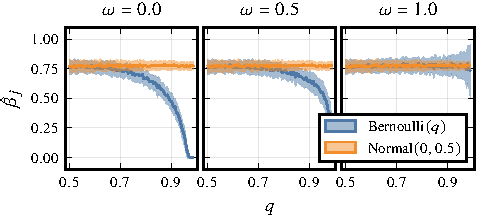
\includegraphics{mixed_data_elnet_small.pdf}
  \caption{%
    Weighted elastic net estimates for \(\alpha = 0.5\) for a problem with a binary
    feature with class balance \(q\) (\(\bernoulli(q)\)) and quasi-normal
    with standard deviation 1/2 (\(\normal(0, 0.5)\)). \(\omega\) indicates
    the scaling of the penalty weights.
  }
  \label{fig:mixed-data-elnet}
\end{figure}


\section{Discussion}\label{sec:discussion}

In this paper, we have studied the effects of normalization in ridge regression and the lasso for features that are binary---an issue that has so far been treated with disregarded in the literature. We have discovered the class imbalance of binary features---the proportion of ones and zeros in the features---have a pronounced effect on both lasso and ridge estimates, and that this effect depends on the type of normalization used. For the lasso, for instance, our results show that features with large class imbalances will be regularized heavily, and provided that \(\lambda\) is large enough might stand little chance of being selected, even if the true effect of the feature on the response is large.

We have, however, found that scaling binary features with standard deviation in the case of ridge regression and variance in the case of the lasso mitigates this effect, but that doing so comes at the price of increased variance. This effectively means that the choice of normalization constitutes a bias--variability trade-off with respect to imbalanced binary features.

To study these effects theoretically and in practice, we have introduced the scaling parameterization
\[
  s_j = (q - q^2)^\delta,
\]
which, for instance, includes the cases \(\delta=0\) (no scaling), \(\delta = 1/2\) (standard deviation scaling), and \(\delta=1\) (variance scaling). These, in turn, correspond to standard choices of normalization types for this kind of data. The common variants max--abs and min--max normalization, for instance, in practice correspond to \(\delta = 0\) in the case of binary data, whilst standardization corresponds to \(\delta = 1/2\). As far as we know, scaling with \(\delta=1\) have previously not been considered in the literature nor to any extent that we are aware of in practice.

Our results demonstrate, however, that the choice of \(\delta\) affects the lasso and ridge estimates heavily in many cases. This is particularly true with respect to selective inference, in which case \(\delta=0\) scaling will reduce the chances of finding the true model via the lasso in class-imbalanced settings~(\Cref{sec:experiments-varbias}). But it will also bias the regression coefficients in both the lasso and ridge, which may also lead to suboptimal predictive performance~(\Cref{sec:predictive-performance}).

Both our theoretical results~(\Cref{sec:theory-binary-features}) and experiments~(\Cref{sec:experiments-varbias}) show that the optimal choice of \(\delta\) may depend on the error in the data-generating process, which is typically unknown. As an alternative, we investigated choosing \(\delta\) in a data-driven manner by optimizing over \(\delta\) as if it were a  hyperparameter~(\Cref{sec:experiments-hyperparameter}).

We have also studied the case of mixed data: designs that consist of both binary and normally distributed features. In this setting, our first finding is that there is an implicit relationship between the choice of normalization and the manner in which regularization affects binary viz-a-viz normally distributed features. For instance, the choice of max--abs normaliation carries a specific assumption about how the effect of a binary feature should be compared to that of a normally distributed feature. There is still much uncertainty about how to best handle the mixed data case and no ground truth given that a binary feature can mean any number of things---few of which are directly comparable to a continuous feature.

In our experimental results, we touch briefly on the case of interactions. In this case, it seems that the interaction term between a normal feature and a binary one is more-or-less unaffected by the class balance of the latter~(\Cref{sec:experiments-interactions}). An interesting avenue for future research could be to study this in more detail, both theoretically and empirically. One particular problem with interactions is
that the interaction term depends on the location, and not just the scale, of the normal feature (in this two-feature setting), which may call for conditional normalization strategies. Much remain to be explored in this area.

Finally, note that our theoretical results are limited by several assumptions: 1) a fixed feature matrix \(\mat{X}\), 2) orthogonality between the features, and 3) normal and idependent errors. In future studies, it would be interesting to relax these assumptions and study the effects of normalization in a more general setting. For instance, the assumption of orthogonality could be relaxed to allow for correlated features, which is often the case in practice. This would allow for a more general understanding of the effects of normalization in regularized regression models. We have also limited ourselves to the case of the lasso and ridge regression. Investigating to which extent, if any, the effects we observe generalize to other models as well would yield valuable insights. We have also focused on the case of binary and continuous features here, but we are convinced that the case of categorical features is also of interest and might raise additional challenges with respect to normalization.


% \subsubsection*{Broader Impact Statement}
%
% In this optional section, TMLR encourages authors to discuss possible repercussions of their work,
% notably any potential negative impact that a user of this research should be aware of.
% Authors should consult the TMLR Ethics Guidelines available on the TMLR website
% for guidance on how to approach this subject.

% \subsubsection*{Acknowledgments}
%
% Use unnumbered third level headings for the acknowledgments. All
% acknowledgments, including those to funding agencies, go at the end of the paper.
% Only add this information once your submission is accepted and deanonymized.

\bibliography{normreg}
\bibliographystyle{tmlr}

\appendix

\section{Additional Theory}
\label{sec:additional-theory}

\subsection{Maximum--Absolute and Min--Max Normalization for Normally Distributed Data}%
\label{sec:maxabs-theory}

In \Cref{thm:maxabs-gev}, we show that the scaling factor in the max--abs method converges
in distribution to a Gumbel distribution.

\begin{theorem}
  \label{thm:maxabs-gev}
  Let \(X_1, X_2, \dots, X_n\) be a sample of normally distributed random variables, each with mean \(\mu\) and standard deviation \(\sigma\). Then
  \[
    \lim_{n \rightarrow \infty}\Pr\left(\max_{i \in [n]} |X_i| \leq x\right) = G(x),
  \]
  where \(G\) is the cumulative distribution function of a Gumbel distribution with
  parameters
  \[
    b_n = F_Y^{-1}(1 - 1/n)\quad \text{and} \quad a_n = \frac{1}{n f_Y(\mu_n)},
  \]
  where \(f_Y\) and \(F_Y^{-1}\) are the probability distribution function and quantile
  function, respectively, of a folded normal distribution with mean \(\mu\) and standard
  deviation \(\sigma\).
\end{theorem}

The gist of \Cref{thm:maxabs-gev} is that the limiting distribution of \(\max_{i \in
  [n]}|X_i|\) has expected value \(b_n + \gamma a_n\), where \(\gamma\) is the
Euler-Mascheroni constant, which shows that the scaling factor depends on the sample size.
In \Cref{fig:maxabs-gev}, we observe empirically that the limiting distribution agrees well
with the empirical distribution in expected value even for small values of \(n\).

In \Cref{fig:maxabs-n} we show the effect of increasing the number of observations, \(n\),
in a two-feature lasso model with max-abs normalization applied to both features. The
coefficient corresponding to the Normally distributed feature shrinks as the number of
observation \(n\) increases. Since the expected value of the Gumbel distribution diverges
with \(n\), this means that there's always a large enough \(n\) to force the coefficient in
a lasso problem to zero with high probability.

\begin{figure}[htpb]
  \centering
  \subfigure[Theoretical versus empirical distribution of the maximum absolute value of normally distributed random variables.\label{fig:maxabs-gev}]{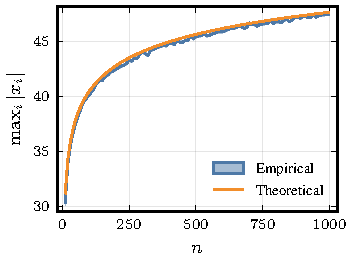
\includegraphics[]{plots/maxabs_gev.pdf}}%
  \hspace{1cm}
  \subfigure[Estimation of mixed features under maximum absolute value scaling\label{fig:maxabs-n}]{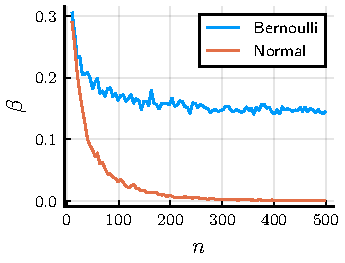
\includegraphics[]{plots/maxabs_n.pdf}}
  \caption{%
    Effects of maximum absolute value scaling
  }
\end{figure}

For min--max normalization, the situation is similar and we omit the details here. The main
point is that the scaling factor is strongly dependent on the sample size, which makes it
unsuitable for normally distributed data in several situations, such as on-line learning
(where sample size changes over time) or model validation with uneven data splits.

\subsection{Solution to the Elastic Net}%
\label{sec:elastic-net-estimator}

Let \((\hat{\beta}_0^{(n)}, \hat{\vec{\beta}}^{(n)})\) be a solution to the problem in
\Cref{eq:elastic-net}. Expanding the function, we have
\[
  \frac{1}{2}\left( \vec y^\T \vec y - 2(\tilde{\mat{X}}\vec{\beta} + \beta_0)^\T\vec{y} + (\tilde{\mat{X}}\vec{\beta} + \beta_0)^\T(\tilde{\mat{X}}\vec{\beta} + \beta_0)\right)
  + \lambda_1 \lVert \vec\beta \rVert_1 + \frac{\lambda_2}{2}\lVert \vec \beta \rVert_2^2.
\]
Taking the subdifferential with respect to \(\vec{\beta}\) and \(\beta_0\), the KKT
stationarity condition yields the following system of equations:
\begin{equation}
  \label{eq:kkt-elasticnet}
  \begin{cases}
    \tilde{\mat{X}}^\T(\tilde{\mat{X}}\vec{\beta} + \beta_0 - \vec{y}) + \lambda_1 g + \lambda_2 \vec\beta \ni \vec{0}, \\
    n \beta_0 + (\tilde{\mat{X}}\vec{\beta})^\T \vec{1} - \vec{y}^\T \vec{1} = 0,
  \end{cases}
\end{equation}
where \(g\) is a subgradient of the \(\ell_1\) norm that has elements \(g_i\) such that
\[
  g_i \in
  \begin{cases}
    \{\sign{\beta_i}\} & \text{if } \beta_i \neq 0, \\
    [-1, 1]            & \text{otherwise}.
  \end{cases}
\]

\subsubsection{Orthogonal Features}

If the features of the normalized design matrix are orthogonal, that is,
\(\tilde{\mat{X}}^\intercal \tilde{\mat{X}} = \diag\left(\tilde{\vec{x}}_1^\T
\tilde{\vec{x}}_1, \dots, \tilde{\vec{x}}_p^\intercal \tilde{\vec{x}}_p\right) \), then
\Cref{eq:kkt-elasticnet} can be decomposed into a set of \(p + 1\) conditions:
%
\[
  \begin{cases}
    \tilde{\vec{x}}_j^\T (\tilde{\vec{x}}_j \beta_j + \ones \beta_0 - \vec{y}) + \lambda_2 \beta_j + \lambda_1 g \ni 0, & j \in [p], \\
    n \beta_0 + (\tilde{\mat{X}}\vec{\beta})^\T \vec{1} -  \vec{y}^\T \ones = 0.
  \end{cases}
\]
%
The inclusion of the intercept ensures that the locations (means) of the features do not
affect the solution (except for the intercept itself). We will therefore from now on assume
that the features are mean-centered so that \(c_j = \bar{\vec{x}}_j\) for all \(j\) and
therefore \(\tilde{\vec{x}}_j^\T \ones = 0\). A solution to the system of equations is then
given by the following set of equations~\citep{donoho1994}:
%
\begin{equation*}
  \hat{\beta}^{(n)}_j = \frac{\st_{\lambda_1}\left(\tilde{\vec{x}}_j^\T \vec{y}\right)}{\tilde{\vec{x}}_j^\T \tilde{\vec{x}}_j + \lambda_2},
  \qquad
  \hat{\beta}_0^{(n)} = \frac{\vec{y}^\T \ones}{n},
\end{equation*}
%
where \(\st_\lambda(z) = \sign(z) \max(|z| - \lambda, 0)\) is the soft-thresholding
operator.

\subsection{Bias and Variance of the Elastic Net Estimator}
\label{sec:bias-var-deriv}

Here, we derive the results in \Cref{sec:theory} in more detail. Let
\[
  {Z_j} = \tilde{\vec{x}}_j^\T \vec{y} = \tilde{\vec{x}}_j^\T(\mat{X}\vec{\beta}^* + \vec{\varepsilon}) = \tilde{\vec{x}}_j^\T (\vec{x}_j\beta_j^* + \boldsymbol{\varepsilon})
  \qquad
  \text{and}
  \qquad
  d_j = s_j(\tilde{\vec{x}}_j^\T \tilde{\vec{x}}_j + \lambda_2)
\]
so that \(\hat{\beta}_j = \st_{\lambda_1}({Z_j})/d_j\). Since \(d_j\) is fixed under our
assumptions, we focus on \(S_{\lambda_1}({Z_j})\). First observe that since \(c_j =
\bar{\bm{x}}_j\),
\[
  \begin{aligned}
    \tilde{\vec{x}}_j^\T \tilde{\vec{x}}_j & = \frac{1}{s_j^2}(\vec{x}_j - c_j)^\T (\vec{x}_j - c_j) = \frac{\vec{x}_j^\T\vec{x}_j - nc_j^2}{s^2_j} = \frac{n \nu_j}{s_j^2}, \\
    \tilde{\vec{x}}_j^\T \vec{x}_j         & = \frac{1}{s_j}(\vec{x}_j^\T \vec{x}_j - \vec{x}_j^\T \ones c_j) = \frac{n \nu_j}{s_j},
  \end{aligned}
\]
where \(\nu_j\) is the uncorrected sample variance of \(\vec{x}_j\). This means that
\begin{equation}
  {Z_j} = \frac{\beta_j^* n \nu_j- \vec{x}_j^\T \vec{\varepsilon}}{s_j}
  \qquad\text{and}\qquad
  d_j = s_j\left(\frac{n \nu_j}{s_j^2} + \lambda_2\right).
\end{equation}
For the expected value and variance of \({Z_j}\) we then have
\begin{align*}
  \E {Z_j}   & = \mu_j = \E \left( \tilde{\vec{x}}_j^\T (\vec{x}_j\beta^*_j + \vec{\varepsilon}) \right)  = \tilde{\vec{x}}_j^\T\vec{x}_j \beta^*_j = \frac{\beta_j^* n \nu_j}{s_j},            \\
  \var {Z_j} & = \sigma_j^2 = \var\left(\tilde{\vec{x}}_j ^\T \vec{\varepsilon}\right) = \tilde{\vec{x}}_j^\T \tilde{\vec{x}}_j\sigma_\varepsilon^2 = \frac{n\nu_j\sigma_\varepsilon^2}{s_j^2}.
\end{align*}

The expected value of the soft-thresholding estimator is
\begin{equation*}
  \E \st_\lambda({Z_j}) = \int_{-\infty}^\infty \st_\lambda(z) f_{Z_j}(z) \du z
  = \int_{-\infty}^{-\lambda}(z + \lambda)f_{Z_j}(z) \du z + \int_{\lambda}^\infty (z - \lambda)f_{Z_j}(z) \du z.
\end{equation*}
And then the bias of \(\hat\beta_j\) with respect to the true coefficient \(\beta_j^*\) is
\begin{equation*}
  \E \hat\beta_j - \beta_j^* = \frac{1}{d_j}\E \st_\lambda({Z_j}) - \beta^*_j.
\end{equation*}

Finally, we note that the variance of the soft-thresholding estimator is
\begin{equation}
  \label{eq:st-variance}
  \var {S_\lambda({Z_j})} = \int_{-\infty}^{-\lambda}(z + \lambda)^2f_{Z_j}(z) \du z + \int_{\lambda}^\infty (z - \lambda)^2 f_{Z_j}(z) \du z - \left(\E \st_\lambda({Z_j})\right)^2
\end{equation}
and that the variance of the elastic net estimator is therefore
\begin{equation*}
  \var \hat\beta_j = \frac{1}{d_j^2} \var \st_\lambda({Z_j}).
\end{equation*}

% \begin{multline*}
%   \E \st_\lambda({Z_j}) = \\
%   \int_{-\infty}^{-\lambda}(z + \lambda)f_{Z_j}(z) \du z + \int_{\lambda}^\infty (z - \lambda)f_{Z_j}(z) \du z
% \end{multline*}
% and
% \begin{multline}
%   \label{eq:st-variance}
%   \var {S_\lambda({Z_j})} = \int_{-\infty}^{-\lambda}(z + \lambda)^2f_{Z_j}(z) \du z \\
%   + \int_{\lambda}^\infty (z - \lambda)^2 f_{Z_j}(z) \du z - \left(\E \st_\lambda({Z_j})\right)^2.
% \end{multline}

\subsubsection{Normally Distributed Noise}%
\label{sec:normally-distributed-noise}

We now assume that \(\vec{\varepsilon}\) is normally distributed. Then
\[
  {Z_j} \sim \normal\left(\mu_j = \tilde{\vec{x}}_j^\T\vec{x}_j \beta_j^*, \sigma_j^2 = \tilde{\vec{x}}_j^\T\tilde{\vec{x}}_j \sigma_\varepsilon^2 \right).
\]
Let \(\theta_j = -\mu_j -\lambda_1 \) and \(\gamma_j = \mu_j - \lambda_1\). Then the
expected value of soft-thresholding of \({Z_j}\) is
\begin{align}
  \E \st_{\lambda_1}({Z_j}) & = \int_{-\infty}^\frac{\theta_j}{\sigma_j} (\sigma_j u - \theta_j) \pdf(u) \du u + \int_{-\frac{\gamma_j}{\sigma_j}}^\infty (\sigma_j u + \gamma_j) \pdf(u) \du u                                               \nonumber                              \\
                            & = -\theta_j \cdf\left(\frac{\theta_j}{\sigma_j}\right) - \sigma_j \pdf\left(\frac{\theta_j}{\sigma_j}\right) + \gamma_j \cdf\left(\frac{\gamma_j}{\sigma_j}\right) + \sigma_j \pdf\left(\frac{\gamma_j}{\sigma_j}\right) \label{eq:mean-centered-eval}
\end{align}
where \(\pdf(u)\) and \(\cdf(u)\) are the probability density and cumulative distribution
functions of the standard normal distribution, respectively. Computing \Cref{eq:st-variance} gives us
\begin{align}
  \label{eq:mean-centered-variance}
  \var{S_\lambda(Z_j)} & = \frac{\sigma_j^2}{2} \left( \erf\left(\frac{\theta_j}{\sigma_j\sqrt{2}}\right) \phantom{-{}} \frac{\theta_j}{\sigma_j}\sqrt{\frac{2}{\pi}} \exp\left(-\frac{\theta_j^2}{2\sigma_j^2}\right) + 1 \right)  \nonumber  \\
                       & \phantom{={}} + 2 \theta_j \sigma_j \pdf \left(\frac{\theta_j}{\sigma_j}\right) + \theta_j^2 \cdf\left(\frac{\theta_j}{\sigma_j}\right) \nonumber                                                                     \\
                       & \phantom{={}} + \frac{\sigma_j^2}{2} \left( \erf\left(\frac{\gamma_j}{\sigma_j\sqrt{2}}\right) - \frac{\gamma_j}{\sigma_j}\sqrt{\frac{2}{\pi}} \exp\left(-\frac{\gamma_j^2}{2\sigma_j^2}\right) + 1 \right) \nonumber \\
                       & \phantom{={}} + 2 \gamma_j \sigma_j \pdf \left(\frac{\gamma_j}{\sigma_j}\right) + \gamma_j^2 \cdf\left(\frac{\gamma_j}{\sigma_j}\right) \nonumber                                                                     \\
                       & \phantom{={}} - \big(\E \st_{\lambda_1}({Z_j})\big)^2.
\end{align}

\subsection{Bias and Variance for Ridge Regression}%
\label{sec:ridge-variance}

\begin{corollary}[Variance in Ridge Regression]
  \label{cor:ridge-variance}
  Assume the conditions of \Cref{thm:classbalance-bias} hold, except that
  \(\lambda_1 = 0\). Then
  \[
    \lim_{q_j \rightarrow 1^+} \var \hat{\beta}_j =
    \begin{cases}
      0                                          & \text{if } 0 \leq \delta < 1/4, \\
      \frac{\sigma_\varepsilon^2 n}{\lambda_2^2} & \text{if } \delta = 1/4,        \\
      \infty                                     & \text{if } \delta > 1/4.
    \end{cases}
  \]
\end{corollary}

\subsection{Centering and Interaction Features}%
\label{sec:centering-interactions}

The main motivation for centering is that it removes correlation between the main features
and the interaction, which would otherwise affect the estimates due to the regularization.
Centering normal features is also important because it ensures that their means do not
factor into the estimation of their effects, which is otherwise the case since the variance
of \(\bm{x}_3\) would then be \(q_1(\sigma^2 + \mu^2(1 - q_1))\) in the case when
\(\bm{x}_1\) is centered and \((q_1 - q_1^2)(\sigma^2 + \mu^2)\) otherwise. Centering
binary features is also important because the variance of the interaction term is otherwise
\(q_1\sigma^2\) (provided \(\bm{x}_2\) is centered), which would mean that the encoding of
values of the binary feature (e.g. \(\{0,1\}\) versus \(\{-1, 1\}\)) would affect the
interaction term.

\subsection{Extended Results on Bias and Variance for Ridge, Lasso, and Elastic Net Regression}%
\label{sec:additional-results-biasvar}

In \Cref{fig:binary-onedim-bias-var-elnet}, we show bias, variance, and mean-squared error
for the weighted elastic net. We see that the behavior of bias as \(q_j \rightarrow 1^+\)
depends on noise level and that there is a bias--variance trade-off with respect to
\(\omega\). As in \Cref{sec:mixed-data}, we modify the weighting factor to have
comparability under \(\kappa = 2\).

\begin{figure}[htpb]
  \centering
  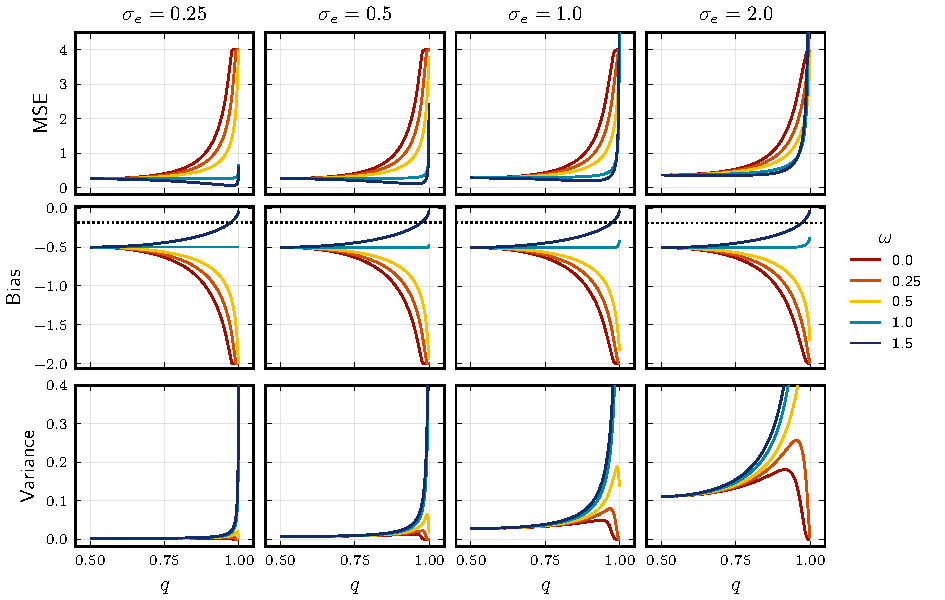
\includegraphics[]{plots/binary_onedim_bias_var_elnet.pdf}
  \caption{%
    Bias, variance, and mean-squared error in the case of the one-dimensional weighted elastic
    net. The measures are shown for different noise levels (\(\sigma_\varepsilon\)), class
    balances (\(q_j\)), and values of (\(\omega\)), which controls the weights that are set to
    \(u_j = v_j = 2\times 4^{\omega - 1}(q-q^2)^\omega\) in order for the results to be
    comparable across different values of \(\omega\). The dotted lines represent the asymptotic
    bias of the estimator in the case of \(\omega = 1\). In the case of \(\omega > 1\), the
    limit of the bias is zero.
  }
  \label{fig:binary-onedim-bias-var-elnet}
\end{figure}

\begin{figure}[htpb]
  \centering
  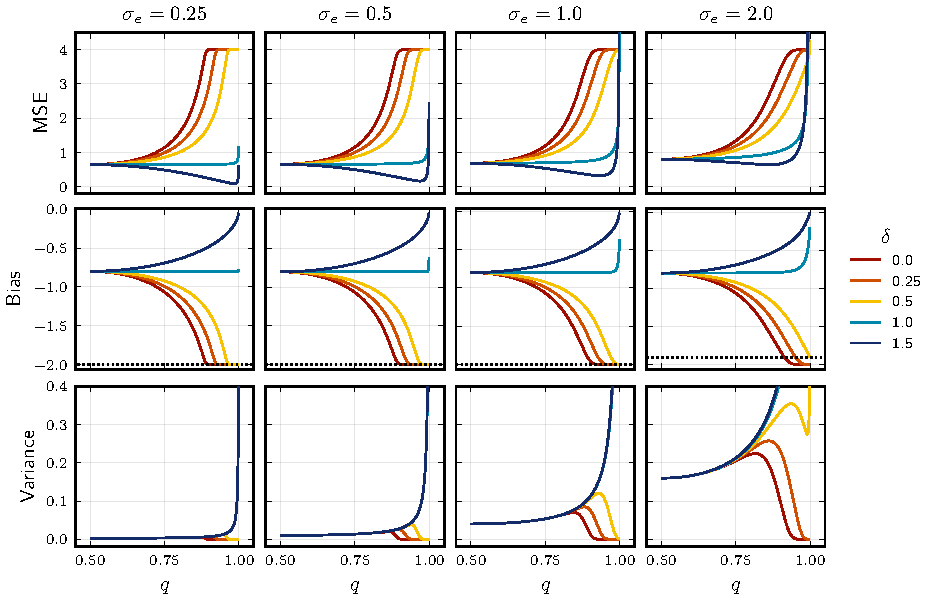
\includegraphics[]{plots/binary_onedim_bias_var_lasso.pdf}
  \caption{%
    Bias, variance, and mean-squared error for a one-dimensional lasso problem,
    parameterized by noise level (\(\sigma_\varepsilon\)), class balance (\(q\)), and
    scaling (\(\delta\)). Dotted lines represent asymptotic bias of the lasso
    estimator in the case when \(\delta = 1/2\).}
  \label{fig:bias-var-onedim-lasso-full}
\end{figure}

\begin{figure}[htpb]
  \centering
  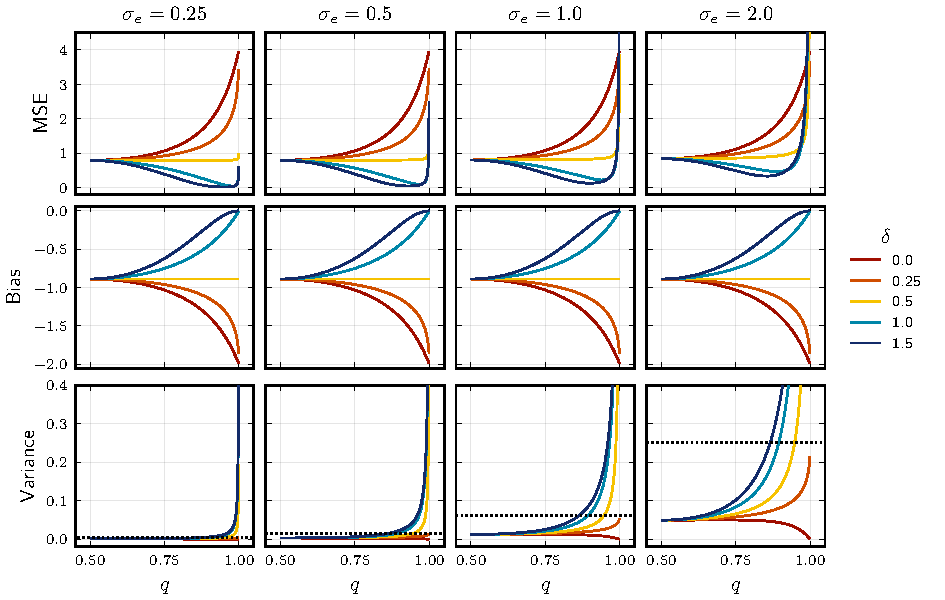
\includegraphics[]{plots/binary_onedim_bias_var_ridge.pdf}
  \caption{%
    Bias, variance, and mean-squared error for one-dimensional ridge regression,
    parameterized by noise level (\(\sigma_\varepsilon\)), class balance (\(q\)), and
    scaling (\(\delta\)). Dotted lines represent asymptotic bias of the ridge
    estimator in the case of \(\delta = 1/4\).}
  \label{fig:bias-var-onedim-ridge-full}
\end{figure}


\section{Proofs}

\subsection{Proof of \Cref{thm:maxabs-gev}}

% TODO: We need to fix notation here. Either use subscript _j everywhere or abuse notation and define
% s = s_j etc.

If \(X_i \sim \normal(\mu, \sigma)\), then \(|X_i| \sim \fnormal(\mu,\sigma)\). By the
Fisher--Tippett--Gnedenko theorem, we know that \((\max_i |X_i| - b_n) / a_n\) converges in
distribution to either the Gumbel, Fréchet, or Weibull distribution, given a proper choice
of \(a_n > 0\) and \(b_n \in \mathbb{R}\). A sufficient condition for convergence to the
Gumbel distribution for a absolutely continuous cumulative distribution
function~\citep[Theorem 10.5.2]{nagaraja2003} is
\[
  \lim_{x \rightarrow \infty} \frac{d}{dx}\left(\frac{1- F(x)}{f(x)}\right) = 0.
\]
We have
\[
  \begin{aligned}
    \frac{1 - F_Y(x)}{f_Y(x)} & = \frac{1 - \frac{1}{2}\erf{\left(\frac{x - \mu}{\sqrt{2\sigma^2}}\right)} - \frac{1}{2}\erf{\left(\frac{x + \mu}{\sqrt{2\sigma^2}}\right)}}{\frac{1}{\sqrt{2\pi\sigma^2}}e^{\frac{-(x-\mu)^2}{2\sigma^2}} + \frac{1}{\sqrt{2\pi\sigma^2}}e^{\frac{-(x+\mu)^2}{2\sigma^2}}} \\
                              & = \frac{2 - \cdf\left(\frac{x - \mu}{\sigma}\right) - \cdf\left(\frac{x + \mu}{\sigma}\right)}{\frac{1}{\sigma}\left(\pdf\left(\frac{x - \mu}{\sigma}\right) + \pdf\left(\frac{x + \mu}{\sigma}\right)\right)}                                                              \\
                              & \rightarrow \frac{\sigma(1 - \cdf(x))}{\pdf(x)} \text{ as } n \rightarrow n,
  \end{aligned}
\]
where \(\pdf\) and \(\cdf\) are the probability distribution and cumulative density
functions of the standard normal distribution respectively. Next, we follow \citet[example
  10.5.3]{nagaraja2003} and observe that
\[
  \frac{d}{dx} \frac{\sigma(1 - \cdf(x))}{\pdf(x)} = \frac{\sigma x (1 - \cdf(x))}{\pdf(x)} - \sigma \rightarrow 0 \text{ as } x \rightarrow \infty
\]
since
\[
  \frac{1 - \cdf(x)}{\pdf(x)} \sim \frac{1}{x}.
\]
In this case, we may take \(b_n = F_Y^{-1}(1 - 1/n)\) and \(a_n = \big(n
f_Y(b_n)\big)^{-1}\).

\subsection{Proof of \Cref{thm:classbalance-bias}}\label{sec:classbalance-bias-proof}

To avoid excessive notation, we allow ourselves to abuse notation and will drop the
subscript \(j\) everywhere in this proof, allowing \(\beta^*\), \(s\), and so on to
respectively denote \(\beta^*\), \(s_j\) et cetera.

Since \(s = (q - q^2)^\delta\), we have
\begin{align*}
  \mu    & = \beta^* n (q - q^2)^{1 - \delta},                      & \frac{\theta}{\sigma} & = -a \sqrt{q - q^2} - b (q - q^2)^{\delta - 1/2},                                          \\
  \sigma & = \sigma_\varepsilon \sqrt{n} (q - q^2)^{1/2 - \delta},  & \frac{\gamma}{\sigma} & = a \sqrt{q - q^2} - b (q - q^2)^{\delta - 1/2},                                           \\
  d      & = n (q - q^2)^{1 - \delta} + \lambda_2 (q - q^2)^\delta, & \frac{\theta}{d}      & = \frac{-\beta^*n - \lambda_1 (q - q^2)^{\delta - 1}}{n + \lambda_2(q-q^2)^{2\delta - 1}}, \\
  \theta & = -\beta^* n (q - q^2)^{1-\delta} - \lambda_1,           & \frac{\gamma}{d}      & = \frac{\beta^*n - \lambda_1 (q - q^2)^{\delta - 1}}{n + \lambda_2(q-q^2)^{2\delta - 1}},  \\
  \gamma & = \beta^* n (q - q^2)^{1-\delta} - \lambda_1,
\end{align*}
with
\[
  a = \frac{\beta^* \sqrt{n}}{\sigma_\varepsilon} \qquad \text{and} \qquad b = \frac{\lambda_1}{\sigma_\varepsilon \sqrt{n}}.
\]

We are interested in
\begin{equation}
  \label{eq:eval-qlimit}
  \lim_{q \rightarrow 1^+} \E \hat{\beta} =\lim_{q \rightarrow 1^+}\frac{1}{d}\left(-\theta \cdf\left(\frac{\theta}{\sigma}\right) - \sigma \pdf\left(\frac{\theta}{\sigma}\right) + \gamma \cdf\left(\frac{\gamma}{\sigma}\right) + \sigma \pdf\left(\frac{\gamma}{\sigma}\right)\right).
\end{equation}
Before we proceed, note the following limits, which we will make repeated use of throughout the proof.
\begin{equation}
  \label{eq:eval-sigma-limits}
  \lim_{q \rightarrow 1^+} \frac{\theta}{\sigma} = \lim_{q \rightarrow 1^+} \frac{\gamma}{\sigma} =
  \begin{cases}
    -\infty & \text{if } 0 \leq \delta < \frac{1}{2}, \\
    -b      & \text{if } \delta = \frac{1}{2},        \\
    0       & \text{if } \delta > \frac{1}{2},
  \end{cases}
\end{equation}

Starting with the terms involving \(\cdf\) inside the limit in \Cref{eq:eval-qlimit}, for
now assuming that they are well-defined and that the limits of the remaining terms also
exist seperately, we have
\begin{align}
  \lim_{q \rightarrow 1^+} \left(-\frac{\theta}{d} \cdf\left(\frac{\theta}{\sigma}\right) + \frac{\gamma}{d} \cdf \left(\frac{\gamma}{\sigma}\right)\right)
   & = \lim_{q \rightarrow 1^+} \Bigg(\left(\frac{\beta^* n}{n + \lambda_2 (q-q^2)^{2\delta - 1}} + \frac{\lambda_1}{n(q-q^2)^{1-\delta} + \lambda_2 (q-q^2)^{\delta}} \right) \cdf \left(\frac{\theta}{\sigma}\right)  \nonumber                                                                                                                                                                                    \\
   & \phantom{= \lim_{q \rightarrow 1^+} \Bigg( } + \left(\frac{\beta^* n}{n + \lambda_2 (q-q^2)^{2\delta - 1}} - \frac{\lambda_1}{n(q-q^2)^{1-\delta} + \lambda_2 (q-q^2)^{\delta}} \right)\cdf \left(\frac{\gamma}{\sigma}\right) \Bigg) \nonumber                                                                                                                                                                 \\
   & = \lim_{q \rightarrow 1^+} \frac{\beta^*n}{n + \lambda_2 (q-q^2)^{2\delta - 1}}\left(\cdf \left(\frac{\theta}{\sigma}\right) + \cdf \left(\frac{\gamma}{\sigma}\right) \right)                                                                                                                                                                                                                        \nonumber \\
   & \phantom{={}} +  \lim_{q \rightarrow 1^+}\frac{\lambda_1}{n(q-q^2)^{1-\delta} + \lambda_2(q -q^2)^{\delta}} \left(\cdf \left(\frac{\theta}{\sigma}\right) - \cdf \left(\frac{\gamma}{\sigma}\right)\right). \label{eq:eval-qlimit-terms}
\end{align}
Considering the first term in \Cref{eq:eval-qlimit-terms}, we see that
\[
  \lim_{q \rightarrow 1^+} \frac{\beta^*n}{n + \lambda_2 (q-q^2)^{2\delta - 1}}\left(\cdf \left(\frac{\theta}{\sigma}\right) + \cdf \left(\frac{\gamma}{\sigma}\right) \right)  =
  \begin{cases}
    0                                          & \text{if } 0 \leq \delta < 1/2, \\
    \frac{2n \beta^*}{n + \lambda_2} \cdf (-b) & \text{if } \delta = 1/2,        \\
    \beta^*                                    & \text{if } \delta > 1/2.
  \end{cases}
\]
For the second term in \Cref{eq:eval-qlimit-terms}, we start by observing that if \(\delta
= 1\), then \((q - q^2)^{\delta - 1} = 1\), and if \(\delta > 1\), then
\(\lim_{q\rightarrow 1^+}(q - q^2)^{\delta - 1} = 0\). Moreover, the arguments of \(\cdf\)
approach 0 in the limit for \(\delta \geq 1\), which means that the entire term vanishes in
both cases (\(\delta \geq 1\)).

For \(0 \leq \delta < 1\), the limit is indeterminite of the form \(\infty \times 0\). We
define
\[
  f(q) = \cdf \left(\frac{\theta}{\sigma}\right) - \cdf \left(\frac{\gamma}{\sigma}\right)
  \qquad\text{and}\qquad
  g(q) = n(q - q^2)^{1-\delta} + \lambda_2(q - q^2)^\delta,
\]
such that we can express the limit as \(\lim_{q \rightarrow 1^+}f(q)/g(q)\). The
corresponding derivatives are
\[
  \begin{aligned}
    f'(q) & = \left(-\frac{a}{2}(1-2q)(q - q^2)^{-1/2} - b(\delta - 1/2)(1-2q)(q - q^2)^{\delta - 3/2}\right)\pdf\left(\frac{\theta}{\sigma}\right)                \\
          & \phantom{= {}} - \left(\frac{a}{2}(1-2q)(q - q^2)^{-1/2} - b(\delta - 1/2)(1-2q)(q - q^2)^{\delta - 3/2}\right)\pdf\left(\frac{\gamma}{\sigma}\right), \\
    g'(q) & = n(1 - \delta)(1-2q)(q - q^2)^{-\delta} + \lambda_2 \delta(1 - 2q) (q - q^2)^{\delta - 1}
  \end{aligned}
\]
Note that \(f(q)\) and \(g(q)\) are both differentiable and \(g'(q) \neq 0\) everywhere in
the interval \((1/2, 1)\). Now note that we have
\begin{multline}
  \label{eq:eval-qlimit-secondterm}
  \frac{f'(q)}{g'(q)} = \frac{1}{n(1-\delta)(q-q^2)^{1/2-\delta} + \lambda_2 \delta (1-2q)(q - q^2)^{\delta-1/2}} \\
  \times \left(-\left(\frac{a}{2} + b(\delta - 1/2)(q - q^2)^{\delta - 1}\right)\pdf\left(\frac{\theta}{\sigma}\right) - \left(\frac{a}{2} - b(\delta - 1/2)(q - q^2)^{\delta - 1}\right)\pdf\left(\frac{\gamma}{\sigma}\right) \right).
\end{multline}
For \(0 \leq \delta < 1/2\), $\lim_{q \rightarrow 1^+}f'(q)/g'(q) = 0$ since the exponential terms of \(\pdf\) in \Cref{eq:eval-qlimit-secondterm} dominate in the limit.

For \(\delta = 1/2\), we have
\[
  \lim_{q \rightarrow 1^+} \frac{f'(q)}{g'(q)} = -\frac{a}{n + \lambda_2} \lim_{q \rightarrow 1^+}\left(\pdf\left(\frac{\theta}{\sigma}\right) + \pdf\left(\frac{\gamma}{\sigma}\right)\right) = -\frac{2a \pdf(-b)}{n + \lambda_2}
\]
so that we can use L'Hôpital's rule to show that the second term in
\Cref{eq:eval-qlimit-terms} becomes
\begin{equation}
  \label{eq:eval-qlimit-stdcase}
  -\frac{2\beta^*\lambda_1\sqrt{n}}{\sigma_\varepsilon(n + \lambda_2)} \pdf\left(\frac{-\lambda_1}{\sigma_\varepsilon\sqrt{n}}\right).
\end{equation}

For \(\delta > 1/2\), we have
\[
  \begin{aligned}
    \lim_{q \rightarrow 1^+} \frac{f'(q)}{g'(q)} & = \lim_{q \rightarrow 1^+} \frac{-\frac{a}{2}\left(\pdf\left(\frac{\theta}{\sigma}\right) + \pdf\left(\frac{\gamma}{\sigma}\right)\right)}{n(1-\delta)(q - q^2)^{1/2 - \delta} + \lambda_2 \delta(1 - 2q)(q - q^2)^{\delta - 1/2}}                                                       \\
                                                 & \phantom{= {}} + \lim_{q \rightarrow 1^+} \frac{b(\delta - 1/2)\left(\pdf\left(\frac{\gamma}{\sigma}\right) - \pdf\left(\frac{\theta}{\sigma}\right)\right)}{n(1 - \delta)(q - q^2)^{3/2 - 2\delta} + \lambda_2 \delta (1 - 2q)(q - q^2)^{1/2}}                                          \\
                                                 & = 0 + \lim_{q \rightarrow 1^+} \frac{b(\delta - 1/2) e^{-\frac{1}{2}\left(a^2(q - q^2) + b^2(q - q^2)^{2\delta - 1}\right)}\left(e^{-ab(q-q^2)^\delta} - e^{ab(q-q^2)^\delta}\right)}{\sqrt{2\pi}\left(n(1-\delta)(q - q^2)^{3/2 - 2\delta} + \lambda_2\delta(1-2q)(q-q^2)^{1/2}\right)} \\
                                                 & = 0
  \end{aligned}
\]
since the exponential term in the numerator dominates.

Now we proceed to consider the terms involving \(\pdf\) in \Cref{eq:eval-qlimit}. We have
\begin{equation}
  \label{eq:eval-qlimit-pdfterm}
  \lim_{q \rightarrow 1^+} \frac{\sigma}{d} \left(\pdf \left(\frac{\gamma}{\sigma}\right) - \pdf \left(\frac{\theta}{\sigma}\right)\right)
  = \sigma_\varepsilon \sqrt{n} \lim_{q \rightarrow 1^+} \frac{ \pdf\left(\frac{\gamma}{\sigma}\right) - \pdf\left(\frac{\theta}{\sigma}\right)}{n(q-q^2)^{1/2} + \lambda_2(q - q^2)^{2\delta - 1/2}}
\end{equation}
For \(0 \leq \delta < 1/2\), we observe that the exponential terms in \(\pdf\) dominate in the limit, and so we can distribute the limit and consider the limits of the respective terms individually, which both vanish.

For \(\delta \geq 1/2\), the limit in \Cref{eq:eval-qlimit-pdfterm} has an indeterminate
form of the type \(\frac{0}{0}\). Define
\[
  u(q) = \pdf\left(\frac{\gamma}{\sigma}\right) - \pdf\left(\frac{\theta}{\sigma}\right)
  \qquad\text{and}\qquad
  v(q) = n(q - q^2)^{1/2} + \lambda_2 (q - q^2)^{2\delta - 1/2}
\]
which are both differentiable in the interval \((1/2, 1)\) and \(v'(q) \neq 0\) everywhere
in this interval. The derivatives are
\[
  \begin{aligned}
    u'(q) & = -\pdf\left(\frac{\gamma}{\sigma}\right)\frac{\gamma}{\sigma} \left(\frac{1}{2}\left(a(1-2q)(q - q^2)^{-1/2}\right) - b(\delta - 1/2)(1- 2q)(q - q^2)^{\delta - 3/2}\right)                 \\
          & \phantom{= {}} + \pdf\left(\frac{\theta}{\sigma}\right) \frac{\theta}{\sigma} \left(\frac{1}{2}\left(a(1-2q)(q - q^2)^{-1/2}\right) + b(\delta - 1/2)(1- 2q)(q - q^2)^{\delta - 3/2}\right), \\
    v'(q) & = \frac{n}{2} (1 - 2q)(q - q^2)^{-1/2} + \lambda_2(2\delta - 1/2)(1 - 2q)(q - q^2)^{2\delta - 3/2}.
  \end{aligned}
\]
And so
\begin{equation}
  \begin{split}
    \frac{u'(q)}{v'(q)} = \frac{1}{n + \lambda_2(4\delta - 1)(q - q^2)^{2\delta - 1}}  \Bigg( & \left(a - b(2\delta - 1)(q - q^2)^{\delta - 1}\right) \pdf\left(\frac{\gamma}{\sigma}\right) \frac{\gamma}{\sigma} \\ & + \left(a + b(2\delta - 1)(q - q^2)^{\delta - 1}\right)\pdf\left(\frac{\theta}{\sigma}\right) \frac{\theta}{\sigma}\Bigg).
  \end{split}
\end{equation}
Taking the limit, rearranging, and assuming that the limits of the separate terms exist, we obtain
\begin{multline}
  \label{eq:eval-qlimit-pdfterm-split}
  \lim_{q \rightarrow 1^+} \frac{u'(q)}{v'(q)} = a \lim_{q \rightarrow 1^+}  \frac{1}{n + \lambda_2 (4 \delta - 1)(q - q^2)^{2\delta - 1}} \left( \pdf\left(\frac{\gamma}{\sigma}\right)\frac{\gamma}{\sigma} - \pdf\left(\frac{\theta}{\sigma}\right)\frac{\theta}{\sigma}\right) \\
  + b (2\delta - 1) \lim_{q \rightarrow 1^+} \frac{1}{n + \lambda_2 (4 \delta - 1)(q - q^2)^{2\delta - 1}} \bigg( \pdf\left(\frac{\gamma}{\sigma}\right) \left(a(q -q^2)^{\delta - 1/2}- b(q - q^2)^{2\delta - 3/2} \right) \\
  - \pdf\left(\frac{\theta}{\sigma}\right) \left(-a(q - q^2)^{\delta - 1/2} - b(q - q^2)^{2\delta - 3/2}\right) \bigg).
\end{multline}
For \(\delta = 1/2\), we have
\[
  \lim_{q \rightarrow 1^+} \frac{u'(q)}{v'(q)} = -\frac{a}{n + \lambda_2}\left(-b \pdf(-b) - b \pdf(-b)\right) + 0 = 2ab \pdf(-b) = \frac{2 \beta^* \lambda_1}{\sigma_\varepsilon^2(n + \lambda_2)} \pdf \left(\frac{-\lambda_1}{\sigma_\varepsilon\sqrt{n}}\right).
\]
Using L'Hôpital's rule, \Cref{eq:eval-qlimit-pdfterm} must consequently be
\[
  \frac{2 \beta^* \lambda_1\sqrt{n}}{\sigma_\varepsilon(n + \lambda_2)} \pdf \left(\frac{-\lambda_1}{\sigma_\varepsilon\sqrt{n}}\right),
\]
which cancels with \Cref{eq:eval-qlimit-stdcase}.

For \(\delta > 1/2\), we first observe that the first term in
\Cref{eq:eval-qlimit-pdfterm-split} tends to zero due to \Cref{eq:eval-sigma-limits} and
the properties of the standard normal distribution. For the second term, we note that this
is essentially of the same form as \Cref{eq:eval-qlimit-secondterm} and that the limit is
therefore 0 here.

\subsection{Proof of \Cref{thm:classbalance-variance}}

The variance of the elastic net estimator is given by
\begin{multline}
  \label{eq:varthm-var}
  \var \hat{\beta}_j = \frac{1}{d^2}\Bigg( \frac{\sigma^2}{2}\bigg(2 + \erf\left(\frac{\theta}{\sigma \sqrt{2}}\right) - \frac{\theta}{\sigma}\sqrt{\frac{2}{\pi}} \exp\left(-\frac{\theta^2}{2\sigma^2}\right) + \erf\left(\frac{\gamma}{\sigma\sqrt{2}}\right) - \frac{\gamma}{\sigma} \sqrt{\frac{2}{\pi}} \exp\left(- \frac{\gamma^2}{2\gamma^2}\right)\bigg) \\
  + 2\theta\sigma \pdf\left(\frac{\theta}{\sigma}\right) + \theta^2 \cdf\left(\frac{\theta}{\sigma}\right) + 2\gamma \sigma \pdf\left(\frac{\gamma}{\sigma}\right) + \gamma^2 \cdf\left(\frac{\gamma}{\sigma}\right) \Bigg)
  - \left(\frac{1}{d}\E \hat{\beta}_j\right)^2.
\end{multline}
We start by noting the following identities:
\[
  \begin{aligned}
    \theta^2                  & = \left(\beta^* n\right)^2 (q-q^2)^{2-2\delta} + \lambda_1^2 + 2\lambda_1 \beta^* n(q-q^2)^{1-\delta},                \\
    d^2                       & = n^2(q -q^2)^{2 - 2\delta} + 2n\lambda_2 (q-q^2) + \lambda_2^2 (q-q^2)^{2\delta},                                    \\
    \theta \sigma             & =  -\sigma_\varepsilon\left(\beta^* n^{3/2}(q- q^2)^{3/2-2\delta} + \sqrt{n} \lambda_1 (q-q^2)^{1/2 - \delta}\right), \\
    \frac{\theta^2}{\sigma^2} & = a^2(q-q^2) + b^2(q-q^2)^{2\delta - 1} + 2ab (q -q^2)^\delta,                                                        \\
    \frac{\sigma}{d}          & = \frac{\sigma_\varepsilon \sqrt{n}}{n(q-q^2)^\frac{1}{2} + \lambda_2 (q-q^2)^{2\delta - 1/2}}.
  \end{aligned}
\]
Expansions involving \(\gamma\) instead of \(\theta\) have identical expansions up to sign
changes of the individual terms. Also recall the definitions provided in the proof of
\Cref{thm:classbalance-bias}.

Starting with the case when \(0 \leq \delta < 1/2\), we write the limit of
\Cref{eq:varthm-var} as
\begin{align*}
   & \lim_{q \rightarrow 1^+} \var \hat{\beta}_j                                                                                                                                                                                                                                                                                                                                         \\ & = \sigma_\varepsilon^2 n  \lim_{q \rightarrow 1^+} \frac{1}{\left(n(q-q^2)^{1/2} + \lambda_2(q-q^2)^{2\delta - 1/2}\right)^2}\bigg(1 + \erf\left(\frac{\theta}{\sigma \sqrt{2}}\right) - \frac{\theta}{\sigma}\sqrt{\frac{2}{\pi}} \exp\left(-\frac{\theta^2}{2\sigma^2}\right)\bigg)                                                                                               \\
   & \phantom{= {}} + \sigma_\varepsilon^2 n  \lim_{q \rightarrow 1^+} \frac{1}{\left(n(q-q^2)^{1/2} + \lambda_2(q-q^2)^{2\delta - 1/2}\right)^2}\bigg(1 + \erf\left(\frac{\gamma}{\sigma\sqrt{2}}\right) - \frac{\gamma}{\sigma} \sqrt{\frac{2}{\pi}} \exp\left(- \frac{\gamma^2}{2\sigma^2}\right)\bigg)                                                                               \\
   & \phantom{= {}}+ \lim_{q \rightarrow 1^+} \frac{2\theta\sigma}{d^2} \pdf\left(\frac{\theta}{\sigma}\right) + \lim_{q \rightarrow 1^+} \frac{\theta^2}{d^2} \cdf\left(\frac{\theta}{\sigma}\right) + \lim_{q \rightarrow 1^+} \frac{2\gamma}{d^2} \sigma \pdf\left(\frac{\gamma}{\sigma}\right) + \lim_{q \rightarrow 1^+}\frac{\gamma^2}{d^2} \cdf\left(\frac{\gamma}{\sigma}\right) \\
   & \phantom{= {}}- \left( \lim_{q\rightarrow 1^+}\frac{1}{d}\E \hat{\beta}_j\right)^2,
\end{align*}
assuming, for now, that all limits exist. Next, let
\[
  \begin{aligned}
    f_1(q) & = 1 + \erf\left(\frac{\theta}{\sigma\sqrt{2}}\right) - \frac{\theta}{\sigma}\sqrt{\frac{2}{\pi}} \exp\left(-\frac{\theta^2}{2\sigma^2}\right) , \\
    f_2(q) & = 1 + \erf\left(\frac{\gamma}{\sigma\sqrt{2}}\right) - \frac{\gamma}{\sigma}\sqrt{\frac{2}{\pi}} \exp\left(-\frac{\gamma^2}{2\sigma^2}\right) , \\
    g(q)   & = \left(n^2(q-q^2) + 2n \lambda_2 (q-q^2)^{2\delta} + \lambda_2^2 (q-q^2)^{4\delta - 1}\right)^2.
  \end{aligned}
\]
And
\begin{align*}
  f_1'(q) & = \frac{\theta^2}{\sigma^2}\sqrt{\frac{2}{\pi}}\exp\left(-\frac{\theta^2}{2\sigma^2}\right),                                    \\
  f_2'(q) & = \frac{\gamma^2}{\sigma^2}\sqrt{\frac{2}{\pi}}\exp\left(-\frac{\gamma^2}{2\sigma^2}\right),                                    \\
  g'(q)   & = (1-2q)\left((q-q^2)^{-1} + 4n\delta \lambda_2 (q-q^2)^{2\delta - 1} + \lambda_2^2 (4 \delta - 1)(q-q^2)^{4\delta - 2}\right).
\end{align*}
\(f_1\), \(f_1\) and \(g\) are differentiable in \((1/2, 1)\) and \(g'(q) \neq 0\) everywhere in this interval. \(f_1/g\) and \(f_2/g\) are indeterminate of the form \(0/0\). And we see that
\[
  \lim_{q \rightarrow 1^+} \frac{f_1'(q)}{g'(q)} = \lim_{q \rightarrow 1^+} \frac{f_2'(q)}{g'(q)} = 0
\]
due to the dominance of the exponential terms as \(\theta/\sigma\) and \(\gamma/\sigma\)
both tend to \(-\infty\). Thus \(f_1/g\) and \(f_2/g\) also tend to 0 by L'Hôpital's rule.
Similar reasoning shows that
\[
  \lim_{q \rightarrow 1^+} \frac{2\theta \sigma}{d^2} \pdf \left(\frac{\theta}{\sigma}\right) = \lim_{q \rightarrow 1^+} \frac{\theta^2}{d^2} \cdf \left(\frac{\theta}{\sigma}\right) = 0.
\]
The same result applies to the respective terms involving \(\gamma\). And since we in
\Cref{thm:classbalance-bias} showed that \(\lim_{q\rightarrow 1^+} \frac{1}{d} \E
\hat{\beta}_j = 0\), the limit of \Cref{eq:varthm-var} must be 0.

For \(\delta = 1/2\), we start by establishing that
\[
  \lim_{q \rightarrow 1^+} \int_{-\infty}^{-\lambda}(z+ \lambda)^2 f_Z(z) \du z = \lim_{q \rightarrow 1^+} \left(\sigma^2 \int_{-\infty}^\frac{\theta}{\sigma} y^2 \pdf(y) \du y + 2 \theta \sigma \int_{-\infty}^\frac{\theta}{\sigma} y \pdf(y) \du y + \theta^2 \int_{-\infty}^\frac{\theta}{\sigma} \pdf(y) \du y\right)
\]
is a positive constant since \(\theta/\sigma \rightarrow -b\), \(\sigma =
\sigma_\varepsilon \sqrt{n}\), \(\theta \rightarrow - \lambda\), and \(\theta\sigma
\rightarrow - \sigma_\varepsilon \sqrt{n}\lambda\). An identical argument can be made in
the case of \(\lim_{q \rightarrow 1^+} \int_{\lambda}^{\infty}(z - \lambda)^2 f_Z(z) \du
z.\) We then have
\[
  \lim_{q \rightarrow 1^+} \frac{1}{d^2} \int_{-\infty}^{-\lambda}(z+ \lambda)^2 f_Z(z) \du z = \frac{C^+}{\lim_{q\rightarrow 1^+} d^2} = \frac{C^+}{0} = \infty,
\]
where \(C^+\) is some positive constant. And because \(\lim_{q\rightarrow 1^+} \frac{1}{d}
\E \hat{\beta}_j = \beta^*\)~(\Cref{thm:classbalance-bias}), the limit of
\Cref{eq:varthm-var} must be \(\infty\).

Finally, for the case when \(\delta > 1/2\), we have
\begin{multline*}
  \lim_{q \rightarrow 1^+} \frac{1}{d^2} \left(\sigma^2 \int_{-\infty}^\frac{\theta}{\sigma} y^2 \pdf(y) \du y + 2 \theta \sigma \int_{-\infty}^\frac{\theta}{\sigma} y \pdf(y) \du y + \theta^2 \int_{-\infty}^\frac{\theta}{\sigma} \pdf(y) \du y\right) \\
  \begin{aligned}
    = \lim_{q \rightarrow 1^+} \Bigg( & \frac{n \sigma^2}{ \left(n (q-q^2)^{1/2} + \lambda_2(q-q^2)^{2\delta - 1/2}\right)^2} \int_{-\infty}^\frac{\theta}{\sigma} y^2 \pdf(y) \du y                                                                                        \\
                                      & - \frac{2\sigma_\varepsilon \sqrt{n}\left(\beta^* n (q- q^2)^{1 - \delta} - \lambda_1\right)}{\left(n(q-q^2)^{3/4 - \delta/2} + \lambda_2(q-q^2)^{3\delta / 2 - 1/4}\right)^2} \int_{-\infty}^\frac{\theta}{\sigma} y \pdf(y) \du y \\
                                      & + \left(\frac{-\beta^*n(q-q^2)^{1-\delta} - \lambda_1}{n(q-q^2)^{1-\delta} + \lambda_2(q-q^2)^\delta}\right)^2 \int_{-\infty}^\frac{\theta}{\sigma} \pdf(y) \du y\Bigg).
  \end{aligned}
\end{multline*}
Inspection of the exponents involving the factor \((q - q^2)\) shows that the first term inside the limit will dominate. And since the upper limit of the integrals, \(\theta/\sigma \rightarrow  0\)  as \(q \rightarrow 1^+\), the limit must be \(\infty\).

\subsection{Proof of \Cref{cor:ridge-variance}}

We have
\begin{equation*}
  \lim_{q\rightarrow 1^+}\var \hat{\beta}_j = \lim_{q \rightarrow 1^+}\frac{\sigma^2}{d^2} \left(\frac{\sigma_\varepsilon \sqrt{n} (q - q^2)^{1/2 - \delta}}{n (q-q^2)^{1 - \delta} + \lambda_2 (q-q^2)^\delta}\right)^2
  = \frac{\sigma_\varepsilon^2 n}{\lambda_2^2} \lim_{q \rightarrow 1^+}(q-q^2)^{1 - 4\delta},
\end{equation*}
from which the result follows directly.

\subsection{Proof of \Cref{thm:weighted-elasticnet-bias}}

Our proof follows a similar structure as in the proof for \Cref{thm:classbalance-bias}
(\Cref{sec:classbalance-bias-proof}). We start by noting the values of some of the
important terms. As before we will drop the subscript \(j\) everywhere to simplify
notation. We have
\begin{align*}
  \mu    & = \beta^*(q -q^2)^\omega,                     & \frac{\theta}{\sigma} & = -a\sqrt{q-q^2} - b(q-q^2)^{\omega - 1/2},                                           \\
  \sigma & = \sigma_\varepsilon \sqrt{n(q-q^2)},         & \frac{\gamma}{\sigma} & = a\sqrt{q-q^2} - b(q-q^2)^{\omega - 1/2},                                            \\
  d      & = n(q-q^2) + \lambda_2(q-q^2)^\omega.\,       & \frac{\theta}{d}      & = \frac{-\beta^*n - \lambda_1(q-q^2)^{\omega - 1}}{n + \lambda_2(q-q^2)^{\omega -1}}, \\
  \theta & = -\beta^*n(q-q^2) - \lambda_1(q-q^2)^\omega, & \frac{\gamma}{d}      & = \frac{\beta^*n - \lambda_1(q-q^2)^{\omega - 1}}{n + \lambda_2(q-q^2)^{\omega -1}},  \\
  \gamma & = \beta^*n(q-q^2) - \lambda_1(q-q^2)^\omega.
\end{align*}

First note the following limit (which is analogous to that in \Cref{eq:eval-sigma-limits}).
\begin{equation}
  \label{eq:eval-sigma-limits-weighted}
  \lim_{q \rightarrow 1^+} \frac{\theta}{\sigma} = \lim_{q \rightarrow 1^+} \frac{\gamma}{\sigma} =
  \begin{cases}
    -\infty & \text{if } 0 \leq \omega < \frac{1}{2}, \\
    -b      & \text{if } \omega = \frac{1}{2},        \\
    0       & \text{if } \omega > \frac{1}{2}.
  \end{cases}
\end{equation}

As in \Cref{sec:classbalance-bias-proof}, we are looking to compute the following limit:
\begin{equation}
  \label{eq:eval-qlimit-weighted}
  \lim_{q \rightarrow 1^+} \E \hat{\beta} =\lim_{q \rightarrow 1^+}\frac{1}{d}\left(-\theta \cdf\left(\frac{\theta}{\sigma}\right) - \sigma \pdf\left(\frac{\theta}{\sigma}\right) + \gamma \cdf\left(\frac{\gamma}{\sigma}\right) + \sigma \pdf\left(\frac{\gamma}{\sigma}\right)\right).
\end{equation}

Starting with the terms involving \(\cdf\) and assuming that the limit can be distributed,
we have
\begin{align}
  \lim_{q \rightarrow 1^+} \left(-\frac{\theta}{d} \cdf\left(\frac{\theta}{\sigma}\right) + \frac{\gamma}{d} \cdf \left(\frac{\gamma}{\sigma}\right)\right)
   & = \lim_{q\rightarrow 1^+} \frac{\beta^* n + \lambda_1(q-q^2)^{\omega -1}}{n + \lambda_2(q-q^2)^{\omega - 1}}\cdf\left(\frac{\theta}{\sigma}\right) \nonumber                \\
   & \phantom{= {}} + \lim_{q\rightarrow 1^+} \frac{\beta^* n - \lambda_1(q-q^2)^{\omega -1}}{n + \lambda_2(q-q^2)^{\omega - 1}}\cdf\left(\frac{\gamma}{\sigma}\right) \nonumber \\
   & =\begin{cases}
        0                              & \text{if } 0 \leq \omega < 1, \\
        \frac{\beta^*n}{n + \lambda_2} & \text{if } \omega = 1,        \\
        \beta^*                        & \text{if } \omega > 1.
      \end{cases} \label{eq:eval-qlimit-terms-weighted}
\end{align}

The derivation of the first case in \Cref{eq:eval-qlimit-terms-weighted} depends on
\(\omega\). For \(0 \leq \omega \leq 1/2\), it stems from the facts that
\(\cdf(\theta/\sigma) \rightarrow 0\) and \(\cdf(\theta/\sigma) \rightarrow 0\) as \(q
\rightarrow 1^+\) together with the existence of the \((q-q^2)^{\omega - 1}\) factor in
both numerator and denominator. For \(1/2 \leq \omega < 1\), the terms cancel each other
out. In the second case, when \(\omega = 1\), the result stems from \(\cdf(\theta/\sigma)\)
and \(\cdf(\gamma/\sigma)\) both tending to 1/2 as \(q \rightarrow 1^+\). And finally for
\(\omega > 1\), the terms involving the \((q-q^2)^{\omega - 1}\) factors vanish and again
the values of the cumulative distribution functions tend to 1/2.

Now, we turn to the terms involving the probability density function \(\pdf\). Again, we
assume the limit is distributive so that
\begin{equation}
  \label{eq:eval-qlimit-pdf-weighted}
  \lim_{q \rightarrow 1^+} \frac{\sigma}{d} \left(\pdf\left(\frac{\gamma}{\sigma}\right) - \left(\frac{\theta}{\sigma}\right)\right) =
  \lim_{q\rightarrow 1^+}\frac{\sigma}{d} \pdf \left(\frac{\gamma}{\sigma}\right) - \lim_{q \rightarrow 1^+} \frac{\sigma}{d} \pdf \left(\frac{\theta}{\sigma}\right).
  % \sigma_\varepsilon \sqrt{n} \lim_{q \rightarrow 1^+} \frac{\pdf\left(\frac{\gamma}{\sigma}\right) - \pdf\left(\frac{\theta}{\sigma}\right)}{n(q-q^2)^{1/2} + \lambda_2(q-q^2)^{\omega - 1/2}}.
\end{equation}
%
Starting with the first term on the right-hand side of \Cref{eq:eval-qlimit-pdf-weighted},
we have
%
\[
  \lim_{q\rightarrow 1^+}\frac{\sigma}{d} \pdf \left(\frac{\gamma}{\sigma}\right) =
  \frac{\sigma_\varepsilon \sqrt{n} \pdf\left(\frac{\gamma}{\sigma}\right)}{n(q-q^2)^{1/2} + \lambda_2(q-q^2)^{\omega - 1/2}}.
\]
For \(0 \leq \omega < 1/2\), this limit is 0 since the exponential terms in the numerator
will dominate as \(q \rightarrow 1^+\). For \(\omega = 1/2\), we have the limit
\(\sigma_\varepsilon\sqrt{n} \pdf(-b)/\lambda_2\). For \(\omega > 1/2\), the limit is
indeterminate of the type \(0/0\). Let
\begin{equation*}
  f_1(q) = \pdf\left(\frac{\gamma}{\sigma}\right)
  \qquad\text{and}\qquad
  g(q) = n(q-q^2)^{1/2} + \lambda_2(q-q^2)^{\omega - 1/2}
\end{equation*}
%
and observe that \(f_1\) and \(g\) are differentiable and \(g'(q) \neq 0 \) for \(q \in
(1/2, 1)\). The derivatives are
%
\begin{align*}
  f_1'(q) & = -\left(\frac{a}{2}(1-2q)(q-q^2)^{-1/2} - b(\omega - 1/2)(1-2q)(q-q^2)^{\omega - 3/2}\right) \frac{\gamma}{\sigma} \pdf\left(\frac{\gamma}{\sigma}\right), \\
  g'(q)   & = \frac{n}{2}(1-2q)(q-q^2)^{-1/2} + \lambda_2(\omega - 1/2)(1-2q)(q-q^2)^{\omega - 3/2}.
\end{align*}
%
Next, we find that
\begin{equation}
  \label{eq:eval-qlimit-pdf-derivative-weighted}
  \frac{f_1'(q)}{g'(q)} = \frac{-a + b(2\omega - 1)(q-q^2)^{\omega - 1}}{n + \lambda_2(2\omega - 1)(q-q^2)^{\omega - 1}} \left(\frac{\gamma}{\sigma}\right) \pdf\left(\frac{\gamma}{\sigma}\right).
\end{equation}
%
Taking the limit of \Cref{eq:eval-qlimit-pdf-derivative-weighted} and invoking L'Hôpital's
rule yields
\[
  \lim_{q\rightarrow 1^+} \frac{f_1'(q)}{g'(q)} =0
\]
both when \(1/2 < \omega < 1\) and \(\omega \geq 1\) since \(\gamma/\sigma\) tends to 0 as
\(q \rightarrow 1^+\) for \(\omega > 1/2\) and the \(\pdf\) term tends to a constant, plus
the fact that the remaining factor in the expression also tends to a constant since the
terms involving \((q-q^2)^{\omega - 1}\) vanish when \(\omega > 1\), are constant when
\(\omega = 1\), and cancel each other out in the limit when \(\omega < 1\).

Finally, if we now consider the second term on the right-hand side of
\Cref{eq:eval-qlimit-pdf-weighted}, set \(f_2(q) = \pdf(\theta/\sigma)\), and perform the
same steps as above, we find that the limits are the same in all cases, which means that
the limits in \Cref{eq:eval-qlimit-pdf-weighted} cancel in the case when \(\omega = 1/2\)
and therefore that
\[
  \lim_{q \rightarrow 1^+} \frac{\sigma}{d} \left(\pdf\left(\frac{\gamma}{\sigma}\right) - \left(\frac{\theta}{\sigma}\right)\right) = 0
\]
for \(0 \leq \omega \). The limit in \Cref{eq:eval-qlimit-weighted} is given by
\Cref{eq:eval-qlimit-terms-weighted}.

\section{Summary of Data Sets}\label{sec:data-summary}

In \Cref{tab:dataset-info} we summarize the data sets we use in our paper.

\begin{table}
  \centering
  \caption{Details of the real datasets used in the experiments, The median \(q\) value
    refers to the median of the proportion of ones for the binary features in the data. Note that in the case of \data{housing}, there is
    only a single binary feature.}
  \label{tab:dataset-info}
  \vskip 0.15in
  \begin{tabular}{
      l
      S[table-format=4.0]
      S[table-format=4.0]
      l
      l
      S[table-format=1.3,round-mode=places,round-precision=3]
    }
    \toprule
    Dataset   & {\(n\)} & {\(p\)} & Response   & Design     & {Median \(q\)} \\
    \midrule
    a1a       & 1605    & 123     & binary     & binary     & 0.970093       \\
    w1a       & 2477    & 300     & binary     & binary     & 0.976181       \\
    rhee2006  & 842     & 361     & continuous & binary     & 0.995249       \\
    housing   & 506     & 13      & continuous & mixed      & 0.93083        \\
    leukemia  & 38      & 7129    & binary     & continuous &                \\
    triazines & 186     & 60      & continuous & mixed      & 0.973118       \\
    \bottomrule
  \end{tabular}
\end{table}

We also visualize the distribution of class balance among all the binary features in
\Cref{fig:data-hist-q}. We note that the clas imbalance for these data sets is quite
severe, which is common for data sets, particularly in the high-dimensional regime.

\begin{figure}[htpb]
  \centering
  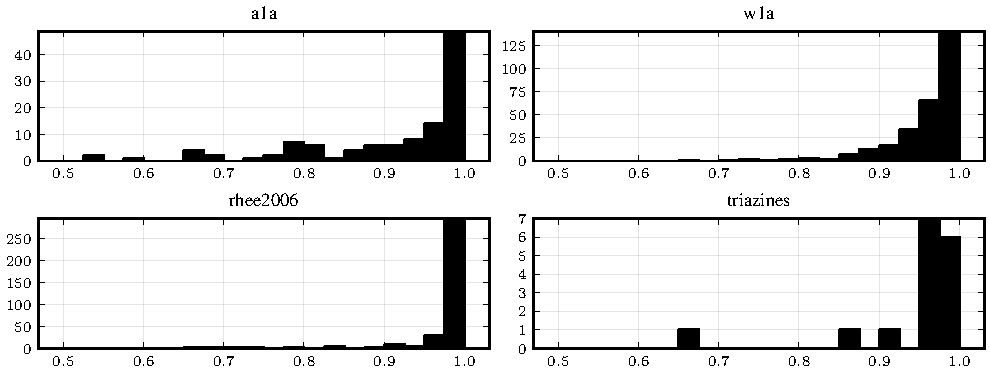
\includegraphics[]{data-hist-q.pdf}
  \caption{%
    Histograms over the distribution of \(q\) (class balance, that is, the
    proportion of ones) for the binary features in each of the data sets
    used in the paper.
  }
  \label{fig:data-hist-q}
\end{figure}



\end{document}
